\documentclass[twoside]{article}
\usepackage{graphicx}
\graphicspath{ {./Col_esc_Figures/} }
\usepackage{lipsum} % Package to generate dummy text throughout this template
\usepackage{wrapfig}
\usepackage[sc]{mathpazo} % Use the Palatino font
\usepackage{amsmath}
\usepackage[T1]{fontenc} % Use 8-bit encoding that has 256 glyphs
% Line spacing - Palatino needs more space between lines
\usepackage{microtype} % Slightly tweak font spacing for aesthetics
\usepackage{lineno}
\usepackage{putex}
\linespread{1.5} 
\usepackage[hmarginratio=1:1,top=32mm,columnsep=20pt]{geometry} % Document margins
\usepackage{multicol} % Used for the two-column layout of the document
\usepackage[hang, small,labelfont=bf,up,textfont=it,up]{caption} % Custom captions under/above floats in tables or figures
\usepackage{booktabs} % Horizontal rules in tables
\usepackage{float} % Required for tables and figures in the multi-column environment - they need to be placed in specific locations with the [H] (e.g. \begin{table}[H])
\usepackage{hyperref} % For hyperlinks in the PDF
\usepackage{paralist} % Used for the compactitem environment which makes bullet points with less space between them
\usepackage{enumitem}
\usepackage{mathrsfs}
\setlist[itemize]{noitemsep}  %Remove spacing in lists
\usepackage{abstract} % Allows abstract customization
%\renewcommand{\abstractnamefont}{\normalfont\bfseries} % Set the "Abstract" text to bold
%\renewcommand{\abstracttextfont}{\normalfont\small\itshape} % Set the abstract itself to small italic text
\usepackage{newtxtext,newtxmath}
\usepackage{titlesec} % Allows customization of titles
\renewcommand\thesection{\Roman{section}} % Roman numerals for the sections
\renewcommand\thesubsection{\Roman{subsection}} % Roman numerals for subsections
\titleformat{\section}[block]{\large\scshape\centering}{\thesection.}{1em}{} % Change the look of the section titles
\titleformat{\subsection}[block]{\large}{\thesubsection.}{1em}{} % Change the look of the section titles

%\usepackage{fancyhdr} % Headers and footers
%\pagestyle{fancy} % All pages have headers and footers
%\fancyhead{} % Blank out the default header
%\fancyfoot{} % Blank out the default footer
%\fancyhead[C]{RCM $\bullet$ November 18$^{th}$ 2014 $\bullet$ Vol. XXI, No. 1} % Custom header text
%\fancyfoot[RO,LE]{\thepage} % Custom footer text

\begin{document}
\begin{center}
	\textbf{\Large{The impacts of dew-induced foliar shielding on the energy, water and isotope balance of leaves
%(old: Water status of hydrophobic leaves improved by the impact of artificial dew deposition on leaf energy balance)
	}}\\
	~\\
	Cynthia Gerlein-Safdi$^1$, Craig James Sinkler$^2$, Kelly Krispin Caylor$^1$\\
	~\\
	$^1$ Princeton University, Department of Civil and Environmental Engineering, \\E-208 E-Quad, 	Princeton, NJ 08544, USA\\
	$^2$ Rider University, 2083 Lawrenceville Road, Lawrenceville, NJ 08648, USA\\

\end{center}
	~\\
Author for correspondence: \textit{Cynthia Gerlein-Safdi}\\
Tel: \textit{+1-609-865-5428}\\
Email: \textit{cgerlein@princeton.edu}\\
~\\
~\\
\begin{table}[h!]
	\centering
	\begin{tabular}{|l|r|}
		\hline
		\textbf{Total word count} (excluding summary,
references and legends) & 6443 \\\hline
Summary & 198 \\\hline
		Introduction & 1219 \\\hline
		Materials and Methods & 2890   \\\hline
		Results & 476 \\\hline
		Discussion & 1801 (28\% of total) \\\hline
		Acknowledgements & 57  \\
		 \hline \hline
		No. of Figures & 7 (all color except No. 6)\\\hline
		No. of Tables  & 2 \\\hline
		No. of Supporting Information files  & 2 figures (all color)\\\hline
	\end{tabular}
\end{table}\\
%\textit{For Cover Letter (max. 50 words per question):}\\
%\textbf{What hypotheses or questions does this work address?}\\
%We hypothesize that the deposition of water droplets from dew or fog will block part of the energy incident on a leaf.  The reduction of incoming energy induces a significant decrease in transpiration, which in turn affects leaf water status and leaf water isotopes. \\
%\textbf{How does this work advance our current understanding of plant science?}\\
%This study is the first one to quantify, through experiment, the impact of non-meteoric water deposition on the leaf energy and water cycle.  We also present a new protocol for the rapid analysis of leaf samples using a laser spectrometer and an induction module. \\
%\textbf{Why is this work important and timely?}\\
%Foliar uptake of non-meteoric water is an important source of water for many ecosystems. This work challenges prior results by showing that the effect of non-meteoric water on the leaf energy cycle impacts leaf water isotopes with a similar amplitude but opposite direction to foliar uptake. 

\newpage
%----------------------------------------------------------------------------------------
%Summary (max 200 words)
%----------------------------------------------------------------------------------------
\subsection*{Summary}
~\\
\begin{itemize}[noitemsep,nolistsep]
\item The uptake of water from the surface of the leaves, called foliar uptake, is common when rainfall is scarce and non-meteoric water (dew or fog) is the only water source. However, many species have very water repellent leaves. Past studies have not differentiated between the uptake of water and the impact of the droplets on the energy balance of the leaf, which we call `foliar shielding'. 
\item Leaves of the hydrophobic \textit{Colocasia esculenta} were sprayed with isotopically enriched water. We developed a protocol using a laser spectrometer and an induction module for the rapid analysis of leaf samples. The leaf water potential and water isotopes were monitored for different water-stress conditions.
\item Dew-treated leaves exhibited a higher leaf water potential (P < 0.05) and c. 30\% decrease in transpiration rate (P < 0.001) compared to the control. The dew treated leaves also had a depleted water isotopic composition compared to the control (P < 0.001). Three possible mechanisms are proposed for the interaction of water droplets with the leaf energy and water balance.
\item Comparing three previous foliar uptake studies to our results, we conclude that foliar shielding has a comparable yet opposite effect to foliar uptake on leaf water isotopes.%, especially when considering isotopic non-steady-state.
\end{itemize}
~\\
\textbf{\textit{Key words}:} \textit{Colocasia esculenta}, dew, foliar uptake, foliar shielding, induction module, laser spectrometer, leaf energy balance, leaf water isotopes
\newpage
%----------------------------------------------------------------------------------------
%Page 5 and subsequent pages: The text, comprising Introduction (not to exceed 6500 words for a Research Article), Mterials and Methods, Results, Discussion, and Acknowledgments.
%----------------------------------------------------------------------------------------

%\begin{multicols}{2} % Two-column layout throughout the main article text
\begin{linenumbers}
\subsection{Introduction}
%The uptake of carbon dioxide by vegetation is a major sink of CO$_2$ and a factor that will determine future climate. Some studies predict a decrease in carbon uptake from vegetation \cite{Raupach:2013iz} because of a general drying of the southern hemisphere, including some tropical areas \cite{Zhao:2010cp}. A mechanistic understanding of land-atmosphere carbon exchanges at the individual and regional scales is necessary to build a comprehensive carbon budget at the global scale and determine whether one can already observe this decline \cite{Ballantyne:2012bk}. 
%
%Because they have optimal temperature and rainfall conditions for vegetation growth, the tropics play a major role in carbon uptake \cite{Osborne:2012wl}.  However, their future is subject to more debate than any other part of the planet \cite{Cox:2013dn, Huntingford:2013cs} . The difficulty in assessing the response of tropical wet forests to climate change comes from the proximity of the mean annual precipitation (MAP) of these areas to 2000~mm/year. If the MAP is above $\sim$2000~mm/y, the vegetation growth is limited by the lack of sunlight (radiation-controlled ecosystems), while if the MAP is below this level, it is limited by water scarcity (water-controlled ecosystems). The predicted climate changes will bring the MAP in some of these areas from above to below this threshold \cite{Guan:2015hq}. It is therefore crucial for the global modeling effort to assess which areas will be transitioning to water-controlled ecosystems and what implications this will have on their carbon uptake rate.

%At the global scale, climate models predict an increase in the number of drought events in some part of the globe, including in the tropics \cite{Neelin:2003db}. Plants absorb CO$_2$ through their stomata, which are small openings on their leaves. In the process, water vapor may escape through the opened stomata \cite{Buckley:2005bf}. Measuring this flux of water vapor, called transpiration, is therefore an effective method for estimating carbon uptake by vegetation. Severe droughts in tropical areas impact global levels of CO$_2$ not only because of the resulting tree loss, but also because trees shut down their stomata to limit water vapor losses that may induce cavitation and permanent damage. This shutdown results in a decrease in carbon uptake. Only a precise knowledge of the water sources that plants have access to would allow one to predict this shut down with accuracy. 
Non-meteoric water is an important source of water for many plants, because it occurs consistently in all environments. But since it only provides small amounts of water, it is often overlooked in large scale models greater than the ecosystem level. Plants from many different environments have long been known to be using fog \cite{Stanton:2013cr, Eller:2013km, Berry:2014wk} or dew \cite{Andrade:2003ck, Clus:2008eh, Lakatos:2012ja, 2013JGRD..11810225B} through foliar uptake. The literature suggesting the importance of this mechanism is growing and includes a wide range of plant species and areas. 

So far, most studies focused on determining circumstances in which specific plants use foliar uptake as a source of water. Vegetation in dry and fog-prone areas like coastlands \cite{Burgess:2004vm, Stanton:2013cr} or mountain hillsides \cite{Berry:2014gd} have adapted to using fog as their main source of water. Similarly, dew water has been shown to be a major source of water on islands where fresh water is scarce \cite{Clus:2008eh} or by species that have physical features allowing them to collect dew water, like epiphytic bromeliads \cite{Andrade:2003ck} or lichens \cite{Lakatos:2012ja}. Both of these plants grow on other plants, often without any access to soil water. %All those case studies focus on specific plants, particular either by their morphology or the ecosystem they grow in. 

In the present study, we will focus on the interaction of non-meteoric water droplets on the leaf energy balance, which we call `foliar shielding'. It is known that many species have water-repellent leaves \cite{Neinhuis:1997vb} which are not adapted to uptake water. For most plants, non-meteoric water deposition is a source of nuisance as it may freeze and cause damages to the leaf in cold climate, or stagnate and cause rotting and pathogen infection in warm environments \cite{EVANS:1992um}. Leaves that are repeatedly exposed to dew have even been shown to become more water-repellent \cite{Aryal:2009hu}. However, micro-droplets of water will indeed form on the surface of even very hydrophobic leaves. The interaction of these droplets on the leaf energy balance (foliar shielding) has been mentioned in previous work \cite{Limm:2009bx, 2013JGRD..11810225B}, but %it has not yet been studied, despite its potentially large impact on both leaf water resources and leaf water isotopes. 
this study is the first to quantify the impact of this process on leaf water balance and leaf water isotopes. 
 \paragraph{Leaf energy balance ---}Because they are unable to move to the shade, leaves are vulnerable to sun radiation, and they can often be warmer than the surrounding air. The leaf temperature will in turn affect the saturation vapor pressure, isotope fractionation, transpiration, and photosynthesis. Smaller leaves tend to be at a temperature closer to the ambient air, since their boundary layer is thinner. This is the reason why, on a single tree, leaves exposed to the sun are usually smaller than shaded ones. %Leaf size and shape have evolved to optimize photosynthesis and water losses. 
To stay cool, leaves use a combination of re-radiation (transfer of energy to the surroundings), convection (heat loss as cool air moves over the surface of the leaf) and evaporative cooling (evaporation of water inside the leaf into water vapor, which is an exothermic process) \cite{vogel2012}. During a drought, leaves have to preserve water to maintain turgor pressure, which competes with evaporative cooling. In this case, leaves are left with re-radiation and convection to cool themselves down. This is sometimes not enough to maintain a low temperature. If its duration extends for too long, a drought might lead to plant mortality. 

Non-meteoric water can supply the plants with a pool of water that will supplement the scarce leaf water by depositing a layer of small water droplets on the surface of the leaves. This provides a form of externalized evaporative cooling. Moreover, the presence of the droplets will both increase the albedo of the leaves, allowing it to reflect more energy \cite{Pinter:1986wx}, and increase surface roughness, which increases the leaf boundary layer, therefore decreasing the vapor pressure deficit (VPD) and lowering the evaporative demand. This later mechanism was proposed by \cite{Limm:2009bx} to explain how fog suppresses nighttime respiration in redwoods. 

Foliar shielding is therefore directly affecting the water status of the leaf by influencing the leaf energy cycle. Depending on temperature and relative humidity, dew deposition can take from c. 1.5 \cite{Abtew:2012vd} to 6 hours \cite{1957QJRMS..83..322M} after sunrise to completely evaporate from the surface of the leaves. Dew and fog can also form in the late afternoon before sunset \cite{Wilson:1999ft, Kabela:2009hd}. Although neither dew nor fog is usually present at the hottest hour of the day, they can effectively shorten the duration of the water-stressed part of the day. This may significantly help the plant maintain its water status over an extended period of drought \cite{Madeira:2002hs, Proctor:2012bg}. 

Dew formation is usually included in global climate models (GCMs) as it merely involves tracking dry bulb temperatures going below the dewpoint temperature. However, its interaction with vegetation is not commonly taken into account. Non-meteoric water deposition events occur around the world, even in dryland ecosystems \cite{Agam:2006ew}, and may affect large areas at the same time. The small changes in the energy, water and carbon balance of each single leaf can therefore have a large cumulative impact at the ecosystem level. Including this interaction into GCMs would allow modelers to better understand the response of vegetation to climate change and the feedback on CO$_2$ atmospheric concentrations.
\paragraph{Leaf water isotopes}
Foliar shielding will influence leaf water isotopes by decreasing leaf transpiration and leaf water enrichment in heavy isotopes \cite{Farquhar:2006cc, Cernusak:2013fx}. The balance of the stable isotopologues of water has been used for decades to understand plant water fluxes \cite{Allison:1985ho, EHLERINGER:1992wz, Werner:2012fw}, but as the number of water sources and sinks increases, the interpretation of isotope data can become difficult. The effect of foliar shielding on leaf water isotopes is, for example, likely to be opposite to that of foliar uptake of heavy fog or dew \cite{Scholl:2010db}, which will enrich leaf water in heavy isotopes. However, foliar uptake studies have so far not taken foliar shielding into account, even though it likely results in an underestimation of the amount of water uptaken by the leaf.

In this study, we present three experiments that focus on the effects of water droplets deposition at the surface of \textit{Colocasia esculenta} leaves. This specie is native to South East Asian tropical forests but has been cultivated across the world for many centuries under the name of taro. With a contact angle of $\sim$164$^\text{o}$ \cite{Neinhuis:1997vb}, \textit{Colocasia esculenta} is considered to have highly water-repellent leaves. Its leaves can reach a size of up to c. 50~cm in length and c. 40~cm in width. We present the first protocol for the fast analysis of small sized leaf samples, allowing for spatial and temporal high-resolution mapping of the leaf-water properties. Using isotopically-labelled water as well as traditional plant physiology techniques, we confirm that the \textit{Colocasia esculenta} leaves do not uptake water from the surface of the leaves.  So far, few studies have attempted to map leaf isotopes because it is both time and labor intensive. While the number of replica presented in this study was limited by the novelty of the protocol, c. 550 plant samples were analyzed. This number largely exceeds the number of samples analyzed by previous studies focused on spatial patterns of leaf-water isotopes \cite{Gan:2002kz, Santrucek:2006by}. We analyze the spatial patterns of leaf water isotopic enrichment and compare them to three different models. In addition, we show that foliar shielding decreases leaf transpiration and increases water potential, and we present three mechanisms that explain the influence of water droplet deposition on the energy and water cycles of water-repellent leaves. Finally, we compare our results to multiple foliar uptake studies. We conclude that foliar shielding has an opposite and larger effect on leaf isotopes than foliar uptake. It is therefore crucial to include foliar shielding in leaf isotope models to properly interpret isotope data of foliar uptake.
%-------------------------------------------------------------------------------------------------------
\subsection{Materials and Methods}
\subsubsection{The added value of stable isotopes}\label{iso}
Stable isotopes of water hold great potential for resolving transpiration and evaporation fluxes across multiple scales \cite{Griffis:2010jt, Rothfuss:2012ep, Wang:2013ee}. The process of evaporation is accompanied by a high degree of isotopic fractionation that leads to evaporated water with an isotopic composition depleted in the heavy isotopologues ${\text{H}_2}^{18}$O and HD$^{16}$O. %, where D symbolizes deuterium. 
This is due to the difference in vapor pressure of the different isotopologues \cite{Farquhar:2006cc}. Isotopic compositions are commonly expressed in terms of the relative ratios
\begin{equation}\label{delta}
\delta_i = \left(\frac{R_i}{R_{r_i}}-1\right)\times 10^3
\end{equation}
of isotope ratios \cite{Mook}, where $\delta_i$ is expressed in \textperthousand, and the index $i$ stands for either $^{18}$O or D. $\text{R}_{^{18}\text{O}} = [{\text{H}_2}^{18}\text{O}]/[{\text{H}_2}^{16}\text{O}]$ and \mbox{$\text{R}_{\text{D}}~=~[\text{HD}^{16}\text{O}]/[{\text{H}_2}^{16}\text{O}]$} 
are the isotope ratios, while the $R_{r_i}$ are the ratios of the corresponding reference standard.  For water, the reference is the Vienna Standard Mean Ocean Water (VSMOW). 

Because precipitation condenses under conditions of equilibrium fractionation, $\delta^{18}$O and $\delta$D in precipitation evolve along a line with slope c. 8, the global meteoric water line (GMWL) \cite{Voelker:2014bq}.
%The fractionation factor, usually noted $\alpha$, describes the isotopic fractionation associated with a reaction or a phase transition. For example, the isotope fractionation factor of water associated with going from the vapor to the liquid phase is defined as:\mbox{$\alpha={R_i}_{\text{liquid}}/{R_i}_{\text{vapor}}$}. Fractionation factors are mostly dependent on temperature. Many empirical relations are available in the literature \cite{Merlivat:1978hk, Horita:1994uf}
However, kinetic isotope effects associated with differences in diffusivity among the different isotopologues of water can lead to deviations from the GMWL \cite{Farquhar:2006cc}. For example, since HD$^{16}$O diffusivity is greater than that of H$_2$$^{18}$O, the water of a leaf that has undergone heavy transpiration will be more depleted in D than in $^{18}$O (Fig.~\ref{d18O_dD_Concept}). Deuterium excess (d-excess) is a widely used measure of how evaporated a pool of water (ocean, lake, leaf) is and is defined as
$\text{d-excess} = \delta \text{D} - 8 \times \delta^{18}\text{O}.$ The average d-excess for precipitation is c. 10\textperthousand. Lower d-excess values generally indicate that the pool has undergone some evaporation \cite{Brooks:2014hd} (Fig.~\ref{d18O_dD_Concept}). 

Stable isotopes are also very efficient to identify different water sources in plants \cite{EHLERINGER:1992wz}. %Groundwater is usually very depleted in heavy isotopes compared to rainwater, because surface water is continuously evaporating until it reaches the aquifer. It is for example possible to distinguish deep-rooted trees from shallow-rooted bushes by looking at the isotopic composition of their respective transpiration \cite{Flanagan:1991wv}.
Indeed, simple mixing models allow one to separate the composition and the fluxes coming from different sources \cite{Phillips:2001hg}. For this reason, stable isotopes are great natural labels that can be used to track pathways of water within plants without harming them; they have been the method of choice for many studies looking at foliar uptake \cite{Breshears:2008vz, Limm:2009bx, Eller:2013km, Berry:2014bo}. Indeed, non-meteoric water is usually enriched in heavy isotopes \cite{Scholl:2010db}, making it easy to trace even after entering the leaf.

\subsubsection{Experiment 1A: Effects of foliar shielding on leaf isotopes in natural conditions}
Our first experiment examines leaf scale spatial and temporal patterns of water isotopes induced by the presence or the absence of dew under natural conditions. Six bulbs of \textit{Colocasia esculenta} were planted in separate pots. All pots were placed outside and received full sun for four weeks. During this time, all plants were heavily watered with tap water ($\delta^{18}$O~$\simeq$~-5.96~\textperthousand, $\delta$D~$\simeq$~-37.63~\textperthousand) to allow plant growth. Once the six plants reached maturity, watering stopped and the plants were moved to a shaded area to remove any sun exposure differences between the plants. %The area was protected and temperature was usually lower than outside of it. Similarly, relative humidity was usually slightly higher. 

Watering stopped two days before the beginning of the treatment. The upper-leaf surfaces in three of the six pots were misted with isotopically-enriched water ($\delta^{18}$O~$\simeq$~8.85~\textperthousand, $\delta$D~$\simeq$~737.64~\textperthousand) every two days using a spray bottle. Any extra water would run off the leaves, leaving them covered in submillimeter-size droplets, which is approximately the natural size for dew-deposition drops \cite{Defraeye:2013jm}. The misting simulated dew and was always performed around 08:00h. 

The three control pots were not watered and did not receive any mist. To avoid contact between the misted water and the soil in the pots, the surfaces of all pots were covered in wrapping plastic. Six leaves were collected between the beginning of the control/dew treatments and the end of the experiments, three weeks later. The sampling and the analysis are described in Section \ref{tech}.
 
 \subsubsection{Experiment 1B: Effects of foliar shielding on leaf isotopes under high water stress}
Our second experiment was designed to artificially increase the contrast between the control and misted treatments from Experiment 1A. The plants from this former experiment were moved into the laboratory and well watered for multiple weeks to offset any effects from the first experiment. Two leaves of similar size and of the same \textit{Colocasia esculenta} plant were cut at the junction of the petiole and the rachis and left to dry c. 80~cm under a blue light (Eiko 1960 EBW, 500 W, 10500~lumens, color temperature of 4800~K). The entire experiment lasted four hours. During that time, the treated leaf was misted with isotopically-labelled water ($\delta^{18}$O~$\simeq$~8.85~\textperthousand, $\delta$D~$\simeq$~737.64~\textperthousand) every half-hour. The control leaf was left to dry without any intervention. After four hours, samples were collected from both leaves as described in Section \ref{tech}.
 
 \subsubsection{Experiment 2: Effects of foliar shielding on leaf water potential}\label{dry}
In this final experiment, we focused on the effect of water droplet deposition on leaf water potential under high water stressed conditions. One leaf was cut at the junction of the petiole and the rachis and left to dry. Three different water stress conditions were tested here: natural drying (control), high heat drying, and high heat and mist. In the high heat case, the leaf was placed 80 cm under a blue light (Eiko 1960 EBW, 500 W, 10500~lumens, color temperature of 4800~K) and left to dry between 8 and up to 10 hours. In the high heat and mist case, the leaf was also misted with ultra pure water every hour using a spray bottle. Again, surplus water was allowed to runoff, leaving the leaf covered in submillimeter size water droplets. Leaf disks of 1~inch diameter were collected every hour. The surface of each leaf disk was wetted with ultra pure water, immediately sanded with ultra-fine sandpaper (3M, 600 grit sandpaper), and the water potential analyzed on a WP4C (Decagon Devices Inc.). 
%For two leaves, the leaf disks were weighted right before being sanded in order to obtain a leaf water potential-leaf water content curve.

\subsubsection{Isotope analysis}\label{tech}
For the water isotope analysis, each leaf was sampled in 12 to 25 different locations depending on the size of the leaf. All of the sampling points were located on the same half of the leaf and each point consisted of four holes (6~mm diameter) punched next to each other forming a square. Each hole was punched as quickly as possible to avoid evaporation, which would influence the isotopic composition of the neighboring holes. Each leaf disk was then secured in an aluminum foil and inserted in a sealed vial. The entire leaf was sampled in one go. The prepared vials were then stored in the fridge until being analyzed. 

The leaf samples were analyzed using an Induction Module (IM) combined to a Cavity Ring Down Spectrometer (CRDS) L2103-i from Picarro Inc. (Sunnyvale, CA, USA). The IM was set on the `normal leaf' setting: the leaf disks did not appear carbonized and, after being dried in the oven at 60$^{\text{o}}$C for 48~hours, they showed no decline in weight, proving that this setting dried the leaf samples completely. The IM was equipped with a micro-combustion module, which has been proven to efficiently reduce the interferences due to the presence of organics (Kate Dennis, private communication) in water samples extracted from plants \cite{West:2010hxa}. On average, each half-leaf was sampled in c. 18 different locations, which corresponds to c. 73 punched holes. 

The entire sampling and IM analysis process lasted from 1.5 to 2 days per half leaf depending on the size of the leaf, which limited the number of replicas we were able to conduct for this study. However, the number of leaf disks sampled per leaf far exceeded the c. 25 samples per half leaf collected by \cite{Gan:2002kz}. In a different study, \cite{Santrucek:2006by} sampled c. 50 disks per half leaf, but the study was carried out only in one replicate for each of the two treatments because of time and money constraints. The size of our study is therefore a significant improvement on previous efforts to map spatial patterns of leaf water isotopes. In addition, the sampling scheme allowed us to look at the temporal evolution of the spatial patterns, which to the best of our knowledge, had never been done before.

\paragraph{IM-CRDS analysis sequence} The IM has only been available commercially for a few years and the number of published studies making use of it is still very limited \cite{2013JGRD..11810225B}. Here we present the first detailed protocol for the analysis of leaf samples. 

The IM-CRDS analysis sequence was adapted from a protocol developed in \cite{vanGeldern:2012cp} for liquid water samples. Following their notation, Table \ref{sequ} presents the sequence of standards and samples. Six empty vials were run at the beginning of each run. The average water vapor content, $\delta^{18}$O, and $\delta$D for the six vials were measured and introduced in a mixing model that allowed us to retrieve the true isotopic composition of the sample analyzed. Reference water samples were run using the filter paper provided  with the instrument and the same piece of filter paper was reused for all the injections of a single reference water. We found that 3~$\mu$l of reference water was necessary to reproduce the amount of water contained by one punch hole of \textit{Colocasia esculenta}. The data was corrected for drift and memory effects, and it was also rescaled back to VSMOW.%The central vein and the half of the leaf that had not been sampled for IM-CRDS analysis were placed in a vial and the water was extracted using cryogenic vacuum distillation. This water was then analyzed both by Isotope Ratio Infrared Spectrometry (IRIS) and Isotope Ratio Mass Spectrometry (IRMS) for comparison with the IM-CRDS.
\paragraph{IRIS and IRMS analysis}
Ten samples were sent to the Center for Stable Isotope Biogeochemistry at the University of California in Berkeley for IRMS analysis. For the IRMS method, $\delta $D was obtained by chromium combustion using an H/Device (Thermo Finnigan, Bremen). Microliters of water were injected in the H/Device and reduced to H$_2$ gas. The ratio of D/H was then measured on a Thermo Delta Plus mass spectrometer. % with a precision of $\pm$ 0.8~\textperthousand.  
%We use the method described in the Thermo GAS Bench II operating manual, ThermoQuest, Oct 1999. 
 For the $\delta^{18}$O analysis, water from standards and samples were pipetted into glass vials and quickly sealed. The vials were then purged with 0.2\% CO$_2$ in Helium and allowed to equilibrate at room temperature for at least 48 hours. The $^{18}$O in the CO$_2$ was then analyzed by continuous flow using a Thermo Gas Bench II interfaced to a Thermo Delta Plus XL mass spectrometer (Wenbo Yang, private communication). In this H$_2$O-CO$_2$ equilibration method, the dissolved components (organic and/or inorganic) do not affect the values of $\delta^{18}$O \cite{West:2010hxa}.
%Long-term external precision is normally better than  � 0.10�. 
For the IRIS analysis, 1.8~$\mu$l of water was injected into a vaporizer and the vapor was pushed through a MCM with dry air. The concentrations of  H$_2^{16}$O, H$_2^{18}$O and HD$^{16}$O were measured on a laser spectrometer (L2103-i) from Picarro Inc. (Sunnyvale, CA, USA). 

The ten samples analyzed both by IRMS and IRIS were used to calculate the offset between the two techniques. All the samples that had been run exclusively by IRIS or IM-CRDS (and had not been analyzed by IRMS) were then corrected for this offset. The IM-CRDS method has not been widely used yet and protocols and precision analyses are still absent from the scientific literature. To justify the results from the IM-CRDS, we compared the values obtained from the extracted water of the half-leaf analyzed by IRIS to the average leaf water composition obtained using a nearest neighbor interpolation on the half-leaf analyzed by IM-CRDS. For the seven leaves analyzed by IM-CRDS, the average difference between those two methods was 2.6$\pm$0.88\textperthousand~in $\delta^{18}$O (mean~$\pm$~SE) and 3.4$\pm$2.4\textperthousand~ in $\delta$D. One potential source of error comes from the IM-CRDS analyses being conducted on a different half of a leaf than the IRMS analyses. However, the average difference we observed between two halves of the same \textit{Colocasia esculenta} leaf was 0.3$\pm$0.2\textperthousand~in $\delta^{18}$O and 1.9$\pm$1.2\textperthousand~in $\delta$D. The differences between the results obtained with the IM-CRDS and the IRMS are therefore not attributable to the analyses being conducted on different halves of the same leaf. The number of studies making use of the fast analyzing capacity of the IM-CRDS is slowly growing \cite{2013JGRD..11810225B}, but further testing is still clearly necessary before using the IM-CRDS technique as an absolute method. However, our goal in this present study is to compare strongly enriched water samples and the order of the differences presented in the next section are up to two orders of magnitude greater than the error observed for the IM-CRDS. We therefore believe that the IM-CRDS is an appropriate method for our applications.%, as it allowed us to quickly process many small samples, therefore increasing the spatial and temporal resolution of our analysis.

\subsubsection{Linking d-excess and transpiration}\label{model}
While d-excess is commonly used in Atmospheric Science \cite{Risi:2013er} and for interpreting ice core data \cite{2009GeCoA..73.6697L}, it has not been widely used in plant physiology. However, because it combines both deuterium and $^{18}$O, d-excess contains more information than the isotopologues taken separately. Indeed, lower (more negative) d-excess values are associated with higher transpiration rates \cite{Voelker:2014bq}. To interpret d-excess differences in terms of transpiration rates, we link d-excess to steady-state relative humidity. The steady-state enrichment of leaf water $\Delta_E$ above source water is expressed in \cite{Farquhar:2006cc} as
\begin{equation}\label{farq}
	\Delta_E~=~(1+\epsilon^*)[(1+\epsilon_k)(1-h)+h(1+\Delta_v)]-1
\end{equation}
where $h$ is the relative humidity, $\epsilon^*$ is the equilibrium fractionation;  $\epsilon^*$~=~9.2~\textperthousand~(74~\textperthousand) for H${_2}^{18}$O (HDO) at 25$^{\text{o}}$C \cite{Craig:1965wd}. The kinetic fractionation factor, $\epsilon_k$, is taken as
\begin{equation}\label{eps}
	{\epsilon_k}^{{\text{H}_2}^{18}\text{O}}~=~\frac{28.5r_s+18.9r_b}{r_b+r_s}~~\text{and}~~{\epsilon_k}^{\text{HDO}}~=~\frac{16r_s+10r_b}{r_b+r_s}
\end{equation}
for H${_2}^{18}$O and HDO, respectively \cite{Farquhar1989, Farquhar:2006cc}. $r_s$ is the stomatal resistance and it is taken to be constant and equal to 217 s~m$^{-2}$ \cite{Hughes:2014hu}. The resistance of the boundary layer, $r_b$, depends on leaf size and wind speed. Here we choose a constant leaf size of 40~cm and a wind speed of 0.2~m~s$^{-1}$, resulting in an $r_b$~=~1.13~10$^5$~s~m$^{-2}$. $\Delta_v$ is the enrichment of ambient water vapor above source water, which was calculated for a measured air composition of $\delta^{18}$O~=~-17~\textperthousand~and $\delta$D~=~-100~\textperthousand. 

The enrichment relative to a source can be linked back to isotopic compositions expressed in $\delta$ notation through the relative ratios $R$:
\begin{equation}\label{Delta}
\Delta_i = \frac{R_i}{R_{\text{source}}}-1.
\end{equation}
Using Equation~\ref{delta} to express $R_i$ as a function of $\delta_i$, we obtain a relation between $\Delta_i$ and $\delta_i$
\begin{equation}\label{alldelta}
 \delta_i~=~\left[ \frac{(\Delta_i+1)~R_{\text{source}}}{R_{r_i}}-1\right]\times1000.
 \end{equation}
 By replacing $\Delta_i$ in Equation~\ref{alldelta} by its expression from Equation~\ref{farq} and combining the expressions for $\delta^{18}$O and $\delta$D, we obtain an expression for the d-excess as a function of the relative humidity $h$. We solve for $h$, bounding its value between 0 and 1. Assuming that the vapor pressure inside the leaves, ${e_i}$, is at saturation, we may calculate the estimated transpiration rate E (in mmol~m$^{-2}$~s$^{-1}$) as
 \begin{equation}\label{evapo}
 \text{E}=g_s~\frac{ {e_i}^*-h~e_{\text{air}}^*}{\text{P}}.
  \end{equation}
Here, P is the atmospheric pressure taken to be 101.3 kPa and $g_s$ (in mmol~m$^{-2}$~s$^{-1}$) is the stomatal conductance equal to 1/$r_s$. ${e_i}^*$ (in kPa) is the saturated vapor pressure calculated for a leaf temperature of 25$^{\text{o}}$C. $e_{\text{air}}^*$ (in kPa) is the saturated vapor pressure at air temperature, which is also taken to be 25$^{\text{o}}$C. In our analysis, we compare the transpiration rates of dew treated leaves, E$_{\text{dew}}$, and that of control leaves, E$_{\text{control}}$.
% ratio of E$_{\text{dew}}$/E$_{\text{control}}$, expressed in \%, where E$_{\text{dew}}$ and E$_{\text{control}}$ are the transpiration rates for the dew treated and the control leaves, respectively. %In this model, all of the changes in leaf isotopic composition are absorbed by the difference in relative humidity. While this is a simplified description of the processes% linking d-excess and transpiration
%, it allows us to estimate the difference in transpiration rates between the treated and control leaves. 

\subsubsection{Spatial patterns}\label{CGmodel}
Leaf water isotopic composition is often compared to the isotopic composition of freely evaporating water as described by the Craig-Gordon (CG) model \cite{Craig:1965wd}. In this model, the fractionation is driven by the difference of saturation vapor pressure between the interior of the leaf and the atmosphere, and by the difference of diffusivity of the isotopologues. However, this simplistic model has been shown to largely underestimate the actual isotopic enrichment. Two main models have since then been proposed to better describe the complexity of leaf water isotopes patterns. The effect of the backward diffusion of enriched water, a form of P\'eclet effect \cite{Farquhar1993, Barbour:2004bh}, has been shown to improve the prediction of bulk water enrichment, as well as the progressive enrichment of leaf water between the xylem and the sites of evaporation \cite{Gan:2002kz}. The string-of-lakes effect takes into account the progressive enrichment of leaf water along the path of water flow \cite{Yakir:1990em, Helliker:2000ep} and improves the modeling of large scale variations of leaf water enrichment.

The Craig-Gordon model of evaporation is expressed as \cite{Gan:2002kz}
\begin{equation}
\Delta_{\text{CG}}~=~\epsilon_k+\epsilon^*+(\Delta_v-\epsilon_k)~\frac{h~e_{\text{air}}^*}{{e_i}^*},
\end{equation}
with $\Delta_v$ the isotopic enrichment of atmospheric water vapor relative to source water (Eq.~\ref{Delta}). $\epsilon_k$, $r_b$, and ${e_i}^*$ depend on leaf temperature. Using an infrared picture of a \textit{Colocasia esculenta} leaf, we are able to calculate $\Delta_{\text{CG}}$ at each pixel to obtain a map of $\Delta_{CG}$ that we compare to the spatial patterns of the measured isotopic enrichment of leaf water relative to source water ($\Delta_{lw}$, as defined in Eq.~\ref{Delta}). Based on meteorologic data available for the duration of the experiment, pressure and relative humidity were taken to be constant and equal to 1013 hPa and 80\%, respectively.

\subsubsection{Competing effects of foliar uptake and foliar shielding}\label{FU}
To compare the relative effects of foliar uptake and foliar shielding, we analyze the results of three different studies that conducted similar experiments on different species. \cite{Limm:2009bx} looked at a ten different species from the coast redwood ecosystem of California (\textit{Pseudotsuga menziesii} and \textit{Sequoia sempervirens} (conifers), \textit{Polystichum munitum} and \textit{Polystichum californicum} (ferns), \textit{Oxalis oregana} (a short herbaceous), \textit{Arbutus menziesii}, \textit{Gaultheria shallon}, \textit{Vaccinium ovatum}, \textit{Notholithocarpus densiflorus} and \textit{Umbellularia californica} (all evergreen broadleaf)), while \cite{Eller:2013km} focused on \textit{Drimys brasiliensis}, a woody broadleaf evergreen native from Central and South America, and \cite{Berry:2014wk} concentrated on \textit{Abies fraseri} and \textit{Picea rubens}, two montane conifers from the Appalachian Mountains. All the studies conducted glasshouse experiments in which saplings experienced nighttime fog. Leaf samples were collected in the evening before the fogging treatment and in the morning, right after the treatment. Every study used isotopically labeled fog with a different composition ($\delta$D$_{\text{fog}}$ - $\delta$D$_{\text{soil}}$~=~16~\textperthousand~in \cite{Berry:2014wk}, 78~\textperthousand~in \cite{Limm:2009bx} and 712~\textperthousand~in \cite{Eller:2013km}). To compare the different experiments, we normalized the results to reflect the leaf water enrichment that would have been observed if the fog water had been %a $\delta$D 
20~\textperthousand~heavier than soil water, since this is within the range of natural values \cite{Scholl:2010db}. 

\subsubsection{Statistical analysis}\label{stat}
Responses for the different experiments were analyzed using a two-sample t-test (Welch's t-test) with a 5\% significance level. This test has been recognized as a better alternative to the Student's t-test when dealing with groups of unequal sample size or variance \cite{Ruxton:2006ea}. % The tests were all performed using Matlab v.~2014b (Mathworks, Natick, MA, USA). 
In the following, we will report the p-value, P, the test statistics, t, and the degrees of freedom of the test, $\nu$. When comparing the results of the different treatments in Experiments 1A and 1B, we treated the multiple samples collected on each leaf as a single population. \textit{stat} and  \textit{syst} refer to the statistical and the systematic errors, respectively.
%-------------------------------------------------------------------------------------------------------------
\subsection{Results}\label{results}
\subsubsection{Water isotopes} The results of Experiments 1A are presented as maps of the analyzed half leaves (Fig.~\ref{expe1A}). The maps were obtained using an inverse distance interpolation and show the evolution of the d-excess of leaves from the control and misted treatments collected at 0, 12 (dew), 14 (control) and 21 (dew and control) days from the beginning of the experiment. All the maps of $\delta$D and $\delta^{18}$O  (Supporting Information, Fig.s~\ref{expe1A2H} and \ref{expe1A18O}) show a progressive enrichment \cite{Cernusak:2013fx} of leaf water when moving away from the main stem towards the rims of the leaf. The average difference between the center and the rim of the leaf for the five leaves presented is $\Delta^{\text{18}}$O~=~11.1$\pm$1.2~\textperthousand~(mean $\pm$ SE) and $\Delta$D~=~23.9$\pm$3.3~\textperthousand. When comparing the composition of the bulk water at the end of the experiment, the dew-treated leaf exhibits a d-excess higher by c. 63.0\textperthousand~  than the control one (two-sample t-test: t~=~-9.4, $\nu$~=~29, P~<~0.001). There is no statistical difference between the treated and control leaves collected on days 12/14 (difference in mean d-excess~$\simeq$~10.2~\textperthousand~, two-sample t-test: t~=~-1.6, $\nu$~=~35, P~=~0.11).

%\subsubsection{Effects of foliar shielding in high water stress conditions} 

Similar maps were produced for Experiment 1B (Fig.~\ref{expe1B}). In this case, the heat lamp artificially increased the transpiration rate in both the control and the misted leaves, leading to significantly enriched $\delta^{18}$O and $\delta$D values and low d-excess values for both treatments. The d-excess in the control case is c. 173.0~\textperthousand~more negative than for the dew treated leaves (two-sample t-test: t~=~3.9, $\nu$~=~29, P~<~0.001). This experiment was merely an extreme version of Experiment 1A, with the objective of accentuating the contrast between the two treatments. While the high heat treatment led to a strong drying of some areas of the leaf, in particular those far away from the central vein, the significant difference observed between the control and the misted treatments do confirm the results of Experiment 1A.

\subsubsection{Leaf water potential} Experiment 2 looks at the temporal evolution of water potential in artificially drying leaves (Fig.~\ref{expe2}). Strong differences in drying pattern are shown for the misted and drought leaves. In both the control and the high heat and mist cases, the leaf water potential experiences a slow decline, which is well approximated by a linear function. However, the high heat treated leaves experience a faster decline and are better approximated by a parabola. Table~\ref{Dryout} presents the average decline from initial to final leaf water potential for the three different treatments. All the data is normalized for leaf size and drying time. The decline in water potential was c. 64\% smaller in the misted leaves than in the leaves subjected to the same high heat treatment but that did not get sprayed (two-sample t-test: t~=~2.37, $\nu$~=~7, P~<~0.05). The decline observed for misted leaves is not statistically different to the one observed for naturally drying leaves (two-sample t-test: t~=~-1.46, $\nu$~=~6, P~=~0.19). %Without the results of Experiments 1 and 2, that confirmed the leaves' high hydrophobicity, this results could easily be mistaken for a foliar uptake process. 

%Large differences in water potential patterns were also observed as a function of leaf size for the high heat treatment: smaller leaves had a stronger decline in water potential than big leaves did. This difference disappears when the leaf is misted. In order to verify that this leaf size difference was not related to a difference in water repartition within the leaf (on a short time scale, transpiration occurs mainly in the lamina), eight \textit{Colocasia esculenta} leaves of length ranging from 14 to 64~cm were weighted, their veins and lamina (inter-vein tissues) separated and re-weighted before being oven-dried for 48~hours and weighted one last time. On average, veins accounted for 39$\pm$1.1\% (mean $\pm$ SE) and the lamina for 61$\pm$1.1\% of the total leaf water (Fig.~\ref{waterPercent}). These values are uncorrelated with leaf size (R = 0.44, P = 0.26), showing that the size dependent change in water potential in the high heat treatment is due to the process of the drying itself, and not due to pre-existing differences in water distribution.
%------------------------------------------------------------------------------------------------

\subsection{Discussion}

%Dew and fog have been shown to have a direct impact on plants water status through direct uptake of water from the leaves or needles \cite{Stanton:2013cr, Eller:2013km, Clus:2008eh, Lakatos:2012ja, Berry:2014gd, Berry:2014wk}. As mentioned before, \textit{Colocasia esculenta} is native to tropical wetlands and posses highly hydrophobic leaves \cite{Neinhuis:1997vb} that allow the plant to prevent the development of fungus. This is confirmed by Experiments 1A and 1B in which the misted leaves all exhibit lower isotopic enrichment in $^{18}$O and D than the control leaves. This is the sign that none of the highly enriched sprayed water is being uptaken by the leaves, even in artificially dry and hot conditions. 

\subsubsection{Foliar shielding-induced decrease in transpiration}
Treated leaves in Experiments 1A and 1B are all less enriched in heavy isotopes than control ones, despite being sprayed with highly enriched water ($\delta^{18}$O~$\simeq$~8.85~\textperthousand, $\delta$D~$\simeq$~737.64~\textperthousand), which is consistent with a lack of foliar uptake. Foliar shielding is then the only phenomenon inducing differences in leaf water d-excess composition between treated and control leaves. 
%Since dew treated leaves have higher d-excess values in Experiments 1A and 1B, we might conclude that foliar shielding decreased leaf transpiration. Yet, we must first consider two other processes that will also influence the leaf water isotopes. First, the dew droplets might actually penetrate the dew-treated leaves through foliar uptake. However, the sprayed water was highly enriched ($\delta^{18}$O~$\simeq$~8.85~\textperthousand, $\delta$D~$\simeq$~737.64~\textperthousand) compared to the source water %used the grow the plants ($\delta^{18}$O~$\simeq$~-5.96~\textperthousand, $\delta$D~$\simeq$~-37.63~\textperthousand): if foliar uptake had been occurring, the dew treated leaves would have shown an enrichment over the control ones. We observe a decrease in both $\delta^{18}$O and $\delta$D for the dew-treated plant compared to the control, which is consistent with a lack of foliar uptake. Second, depleted source water contained in the soil and stem of the plant is constantly entering the leaf. %because the isotopic composition of the source water is located on the GMWL (see Fig.~\ref{d18O_dD}), its effect would also have been to decrease leaf d-excess. Moreover, 
%We expect this effect has the same impact on both dew treated and control plants, and so we exclude it when interpreting differences between the two treatments. We conclude that foliar shielding is the primary phenomenon impacting leaf water d-excess composition. 
We apply the model described in Section~\ref{model} to interpret our results in terms of the transpiration rate, $E$. 

The use of a constant stomatal conductance and leaf temperature are most likely the largest sources of systematic error in this model. To calculate the systematic error associated with our choices for those parameters, we calculate E$_{\text{dew}}$/E$_{\text{control}}$ for a range of leaf temperatures from 10$^{\text{o}}$ to 40$^{\text{o}}$C and for a stomatal conductance $g_s$ from 0.1 to 0.8~mmol~m$^{-2}$~s$^{-1}$. We find that the systematic error associated with our choice of $g_s$ is negligible, while that associated with the choice of T$_{\text{leaf}}$ is important for Experiment 1A, but nor for Experiment 1B. 

For Experiment 1A, the transpiration rate obtained for the dew treated leaf is significantly lower than that of the control (t~=~-9.4, $\mu$~=~38, P~<~0.0001) by $29.9~{\pm2.6}$~(stat)~${\pm1.1}$~(syst)~\%. %(median $\pm$ statistical error $\pm$ systematic error associated with T$_{\text{leaf}}$. All assuming gaussian errors). 
Similar results were found for Experiment 1B, where the dew treatment significantly (t~=~-3.9, $\mu$~=~29, P~<~0.0001) decreased transpiration by $29.9~{\pm9.1}$~(stat)~\%. %${\pm0.09}$~(syst)~\%. %While those values should be considered more as an order of magnitude than a precise estimate of transpiration decrease,
These values are consistent with \cite{1988BoLMe..45..209G}, who estimated that the reduction in transpiration due to dewfall could reduce daily plant water use by c. 10\%. This value was obtained for wheat plants associated with a low transpiration rate. Since \textit{Colocasia esculenta} leaves are larger and have a higher transpiration rate, we expect the reduction to be larger in our case (see Section~\ref{mechanisms}).
% We conclude that foliar shielding has a significant impact on leaf transpiration rate. 

\paragraph{Spatial patterns}
To understand the spatial patterns observed in Fig.~\ref{expe1A} and \ref{expe1B}, we calculate the expected CG enrichment for $^{18}$O as described in Section~\ref{CGmodel}. We compare the results to the leaf water enrichment above source water, $\Delta_{lw}$ measured for three leaves from Experiment 1A (Fig.~\ref{CG}). All three leaves tested show an enrichment on both side of the 1:1 line, which corresponds to the CG enrichment. %Comparing the ratios $\Delta_{lw}$/$\Delta_{\text{CG}}$ for the three cases, the observed differences between the different leaves are all significant (P<0.0001 in both cases). 

Leaf water depleted from the expected CG model points toward a larger importance of the P\'eclet effect, while samples located across the 1:1 line show a larger importance of the string-of-lakes effect \cite{Gan:2002kz}. \textit{Colocasia esculenta} leaves seem to generally behave like a string-of-lakes, in which the enriched water leftover after transpiration increases the expected enrichment of the next pool. This effect has been shown to be particularly important in monocots, since they tend to have parallel veins with stomata located in-between them that act as enrichment sites \cite{Helliker:2000ep}. Since \textit{Colocasia esculenta} is a monocot itself, our result confirms the main importance of the string-of-lakes effect in monocots and expands previous work that has so far been concentrating on dicots \cite{Yakir:1990em, Gan:2002kz, Santrucek:2006by} and only a few monocots \cite{Helliker:2000ep, Gan:2003ff}. We find a strong linear correlation (R$^2$ = 0.84, P~<~0.001) between $\Delta_{lw}$/$\Delta_{\text{CG}}$ and distance from the petiole (Fig.~\ref{CGdist}). $\Delta_{lw}$/$\Delta_{\text{CG}}$ appears to be smaller than 1 for samples close to the petiole, and larger than 1 at the tip of the leaf and at the rims. This pattern has already be observed in cotton leaves \cite{Gan:2002kz} and was pointed out as another characteristic trait of the string-of lakes effect. 

%While the samples from the dew treated leaf are consistent with a strong string-of-lakes effect, the $\Delta_{lw}$/$\Delta_{\text{CG}}$ is significantly lower than for the control (t~=~185, $\mu$~=~15050, P~<~0.0001) and the initial (t~=~142, $\mu$~=~14883, P~<~0.0001) leaves. The CG model used here is the same for all three leaves, because leaf temperature data was not available for the leaves used in the isotope analysis. We expect the dew leaf to have a lower temperature, which would decrease $\Delta_{\text{CG}}$, bringing the samples closer to the 1:1 line, 



%\begin{equation}
%\Delta_{lw}~=~\Delta_{\text{CG}}~\frac{1-e^{-\mathscr{P}}}{\mathscr{P}},
%\end{equation}
%where $\mathscr{P}$ is the P\'eclet number \mbox{$\mathscr{P}=EL/CD$}. $E$ is the transpiration rate, $L$ is the scaled effective path length of water between the xylem and sites of evaporation, $C$ is the molar concentration of water and $D$ is the diffusivity of H$_2^{18}$O in water. If transpiration is suppressed, the leaf water enrichment should match CG. If transpiration increases, the P\'eclet effect becomes more important and the resulting leaf water will be below the CG enrichment. However, the dew effect is believed to lower transpiration...???

\paragraph{Temporal patterns} 

Leaves collected from both treatments on day 12 or 14 present results that disagree with the trends formed by the results of day 0 and 21 (Fig.~\ref{expe1A}). 
%For the control, d-excess is generally decreasing between day 0 and day 21, but the leaf collected on day 14 shows values of d-excess higher than expected. In the dew treatment case, the general trend is reverse and d-excess at the end of the experiment (day 21) is much higher than on day 0. However, the dew treated leaf collected on day 12 presents lower values of d-excess than expected from this trend. 
It is important to note that the plants were kept outside throughout the experiment and were therefore subjected to the daily variations of temperature and relative humidity, which both influence the transpiration rate as well as the isotopic composition. The dew-treated leaf collected on day 12 was sampled after a prolonged period of dry and hot weather that might have enhanced the transpiration despite the artificial dew treatment. This may explain why this leaf presents lower d-excess values than expected. 
A series of small rain events happened on the day preceding the collection of the first control leaf on day 14, which may have decreased the transpiration rate and increased the d-excess composition of the leaf. %During the experiment, the plants were kept in a shaded, protected area below a building where the temperature is often lower and the relative humidity higher than outside, which lead to natural dew formation on some nights. We believe this to be particularly relevant for the days preceding the collection of the first control leaf on day 14%(see Fig.~\ref{dewpoint})
%. Finally, a series a small rain events happened on the day preceding this collection, which may have decreased the transpiration rate and increased the d-excess composition of the leaf.

%The leaf average isotopic composition of the dew treated and control leaves (see Fig.~\ref{d18O_dD}. Fig.~\ref{d18O_dD_Concept} provides an explanation on how to interpret this figure.) shows that the isotopic composition of the control leaves evolved directly from evaporated source water (tap water), while the dew treated leaves are evolving on a line parallel to the GMWL. Before the treatment started the water in the dew treated leaves most likely followed an evaporation line similar to that of the control leaves. However, after the treatment started, transpiration in the dew treated leaves stopped and the water in those leaves followed a line parallel to the GMWL. For the samples to evolve on such a line, only equilibrium isotopic fractionation is happening within the leaf. Indeed, any kinetic fractionation would induce a slope of less than 8. In terms of leaf physiology, this is the sign that water vapor is not diffusing out of the leaf, i.e. that little transpiration is occurring.  

\subsubsection{Leaf energy cycle}\label{mechanisms}
%Despite the leaf's hydrophobicity, we observed submillimeter size droplets of water attached to the surface of the leaf. 
Our results show that the deposition of submillimeter size droplets allow the leaf to decrease its transpiration rate and maintain its water potential. The water balance of the leaf is influenced by the change in energy balance associated with the water droplets deposited at the surface through three distinct processes. 

First, the deposited droplets increase the albedo of the leaf, allowing more of the radiation to be reflected away from the leaf. %The albedo is the reflection coefficient for solar radiation off natural surfaces. 
Depending on the direction of the incoming solar radiation, water can have an albedo as high as 1 (perfect reflector) whereas typical values for leaves are c. 0.2 for visible light. The increase of vegetation albedo due do dew deposition has been observed in the field many times \cite{Pinter:1986wx, Zhang:2012gy}. By reflecting more radiation when they are wet, leaves will decrease the incoming shortwave radiation and consequently keep their temperatures lower. This will in turn reduce the evaporative demand and the leaf transpiration.

Second, the energy that is not reflected will be dissipated through the evaporation of the droplets. The dissipated energy will not contribute to the leaf energy budget. Moreover, because evaporation is an exothermic process, the evaporation of the water droplets will result in a cooling of the leaf surface. This will again reduce the evaporative demand and the transpiration.
%The energy that is not reflected by the droplets will be used to evaporate them; because of the high heat capacity of water, the evaporation of the droplets will dissipate energy that will not contribute to the leaf energy budget. Moreover, because evaporation is an exothermic process, the evaporation of the water droplets will result in a cooling of the leaf surface. This will again reduce the evaporative demand and the transpiration.

Finally, the evaporation of the droplets will cause the air close to the leaf to have a higher relative humidity than the surrounding air \cite{Defraeye:2013jm}, creating a moist micro-climate around the leaf \cite{jones1992}. This will decrease the difference between the interstitial and the air vapor pressures, and reduce the flux of water vapor out of the leaf, namely transpiration. By decreasing the outward flow of water vapor, more CO$_2$ will be able to enter the leaf, increasing interstitial CO$_2$ concentration, photosynthesis, and water use efficiency. The increase in surface roughness associated with the presence of the droplets at the surface of the leaf will also contribute to increasing the size of the boundary layer.
%the evaporating droplets increase the boundary layer and locally decrease the VPD, creating a moister environment around the leaf. The increase in surface roughness associated with the presence of the droplets at the surface of the leaf will also contribute to increasing the size of the boundary layer. %The leaf size dependency of this third mechanism is confirmed by the leaf size dependent behavior observed for the misted case of Experiment 2 (see Fig.~\ref{expe2}): if only the first two mechanisms were at play, one would not expect a difference between two leaves of different size receiving mist. However, bigger misted leaves will create a larger micro-climate, increasing the length of the boundary layer and therefore decreasing the VPD even further than a small leaf could \cite{Defraeye:2013jm}. This lower VPD then induces a decrease in transpiration and an increase in leaf water potential, as it is the case in Experiment 2. 
Water potential values are correlated with leaf relative water content \cite{Maxwell:1978uw} and with stomatal conductance \cite{Lhomme:1998vo}; by maintaining a higher water potential, the leaf will be able to open its stomata wider. CO$_2$ assimilation is in turn linearly correlated to stomatal conductance \cite{Lambers:2008uw}. As a result, by affecting the leaf energy cycle, foliar shielding will allow the leaf to maintain its water status and increase CO$_2$ assimilation through multiple mechanisms.

\subsubsection{Implications for foliar uptake studies}
By decreasing evaporation, foliar shielding suppresses the isotopic enrichment associated with leaf water transpiration \cite{Farquhar:2006cc}. Therefore, leaves undergoing foliar shielding will have a bulk isotopic composition lower (more depleted) than leaves that do not experience it. The average $\delta$D enrichment between the first and last days of collection for Experiment 1A were -9.1$\pm$3.7~\textperthousand~(mean $\pm$ SE) for the control leaf and -27.9$\pm$2.9~\textperthousand~for the dew treated leaf. This corresponds to a -18.8$\pm$6.6~\textperthousand~difference in enrichment between sprayed and control treatments. In the case of highly water stressed leaves (Experiment 1B, Fig.~\ref{expe1B}), the difference in enrichment reaches -45.2$\pm$35.8~\textperthousand. %In both cases, the dew-treated leaf was more depleted in heavy isotopes than the control. 

Non-meteoric water is usually more enriched in deuterium than rain and soil water by up to $50~\text{\textperthousand}$ \cite{Scholl:2010db}. If foliar uptake is indeed happening in a leaf, the uptake of heavy fog water will then enrich the leaf water, while foliar shielding depletes leaf water in heavy isotopes. \cite{Limm:2009bx} pointed out the tension between foliar uptake and nighttime suppression of respiration due to the saturated atmosphere during fog events. Transpiration is a much larger water loss for plants than respiration and the effects of foliar shielding during day time is expected to be have a even larger impact on leaf isotopes than that discussed by \cite{Limm:2009bx}. 

Using previous studies on foliar uptake (described in Section~\ref{FU}), we were able to compare the relative impact of both processes. Foliar uptake has the largest impact on conifers (Fig. \ref{FU_VS_FS}), where the difference in enrichment between treatment and control reaches up to c. 20~\textperthousand. Foliar shielding for the non-water stressed case (Experiment 1A) exhibits the opposite effect, with a magnitude similar to the largest foliar uptake case. In the water stressed case (Experiment 1B), the depletion observed is as large as c. 45.2~\textperthousand. %The true effect of foliar shielding on leaves in the field during a drought likely lies in between the two cases shown here. 
The three foliar experiments presented here all used nighttime treatment, so foliar shielding did not impact the enrichment observed. However, the competing effects of foliar uptake and foliar shielding are likely to be very important when analyzing field or day time foliar uptake experiment data. For example, \cite{Berry:2014bo} observed a significantly larger enrichment when fogging saplings in the morning than in the afternoon. This results is well explained if foliar shielding is taken into account, since foliar shielding will have a larger effect in the afternoon, when leaves are hotter and radiations stronger.
Our results suggest that, in the field, foliar shielding might have a larger impact on leaf isotopes than foliar uptake. %The relative importance of foliar uptake VS foliar shielding will depend on many factors, including the isotopic composition of the non-meteoric water, the timing and length of the wetting event, the size of the leaf, the atmospheric conditions and of course, the specie. To properly interpret isotope data, future studies on foliar uptake should include foliar shielding into their isotope balance calculation. 

The results of our study show a larger impact of foliar shielding in times of drought than in well-watered conditions. The simultaneous occurrence of non-meteoric water deposition and drought is common in drylands \cite{Agam:2006ew}, where many plants rely on non-meteoric water as their primary source of water \cite{Stanton:2013cr}. %to tropical forests \cite{Lakatos:2012ja}. Indeed, 
Regular dew formation has also been observed in the upper canopy of the Amazon forest during the dry season \cite{Satake:cw, Frolking:2011di}. In those cases, the energy balance is thought to be the main driver of leaf water isotopic composition, with a response much larger than to soil water availability, for example \cite{wayland2014}. 
Foliar shielding will delay the time when leaves reach their maximum transpiration rate and attain isotopic steady state \cite{Dubbert:2014iz}. %Indeed, \cite{Abtew:2012vd} calculated that dew evaporation from the surface of a leaf takes c. 75~min in southern Florida. 
Isotopic steady state is often assumed when interpreting transpiration data, but \cite{Dubbert:2013ew} recently showed that this assumption is typically unjustified and can lead to errors in estimated transpiration fluxes by up to 70\%, since steady state models systematically overestimate the isotopic enrichment of leaf water. %These results are in agreement with the decrease in leaf water enrichment that we observed in leaves experiencing foliar shielding. 
Isotopic steady state depends on the leaf transpiration rate, which changes quickly as energy flux incident on the leaf changes, for example when the leaf goes from the shade to the sun \cite{Smith:2013cf}. Foliar shielding has a large impact at short time scales on both leaf transpiration and water isotopes because of this fast response.
\subsubsection{Conclusion}
In this study, we used the highly hydrophobic leaves of \textit{Colocasia esculenta} to look at the impacts of dew water droplets deposition (called foliar shielding) on the leaf energy, water and isotope balance. We show that the spatial patterns of enrichment are consistent with the string-of-lakes model, which is common in monocots. Our results show that foliar shielding significantly decreases leaf transpiration by c. 30\%, maintains leaf water potential, and limits leaf water isotopic enrichment. We highlight the opposite effects of foliar uptake, which enriches leaf water in heavy isotopes, and foliar shielding, which depletes it. Because both effects are of similar magnitude, taking both processes into accounts  is crucial to properly interpret field data of foliar uptake. %Our results are also in agreement with recent studies pointing at the importance of non-isotopic steady state for the proper understanding of leaf water fluxes. 
%More experiments are now required to understand the effects of foliar shielding on different species and for a range of leaf shapes and sizes. Introducing stable isotopes of water in a model of leaf energy and water balance could help to interpret the competing effects of foliar uptake and foliar shielding, give a new insight into non-steady-state transpiration, and improve the general understanding of the interaction of leaves with their environment.

\subsection*{Acknowledgments}
The authors thank Todd Dawson and Wenbo Yang %from the Center for Stable Isotope Biogeochemistry at the University of California in Berkeley 
for the IRMS analysis, and Fulton Rockwell for the discussion on spatial patterns. C.Gerlein-Safdi and K.K. Caylor acknowledge the financial support of NASA Headquarters under the NASA Earth and Space Science Fellowship Program - Grant 14-EARTH14F-241 - and of the Science, Technology, and Environmental Policy Fellowship from the Princeton Environmental Institute.
%\subsection{Conclusion}

%Dew and fog  commonly occur all around the world and in a wide range of ecosystems, from drylands \cite{Agam:2006ew} to tropical forests \cite{Lakatos:2012ja}. Indeed, regular dew formation has been observed by scatterometer in the upper canopy of the Amazon forest, even during the dry season \cite{Satake:cw, Frolking:2011di}. 
%\cite{Frolking:2011di} observed a sharp decrease in morning backscatter over the Amazon forest for the summer months of 2005, which they associated with a lack of morning dew formation. This summer was known as a mega-drought for the Amazon forest and led to a high tree mortality \cite{Zeng:2008gh}. However, the accumulating water deficit anomaly for that year was just as high as that of the year 2002, which did not experience the same tree mortality. The main difference in water resources between the two years appears to be the presence or absence of dew. 

%In the context of climate change and with an increasing number of drought in some tropical forests, and in particular the Amazon forest \cite{Cook:2014ks}, even a small delay in the beginning of the transpiration in the morning could have a huge impact when spanning over the whole dry season and, for example, the entire Amazon forest. While tropical forests are usually carbon neutral, \cite{Gatti:2015gq} calculated that during the 2010 mega-drought in the Amazon, the basin lost 0.48 PgC.yr$^{-1}$. This corresponds to about 10\% of the amount of anthropogenic carbon released in the atmosphere for that year. Understanding all the aspects of plant functions in topical forests is therefore crucial if we want to better anticipate future climate. Despite its potentially large impact, foliar shielding is yet to be include in climate models. Further investigation is now necessary to quantify the transpiration decrease associated with water droplets deposition, as well as the impact on leaf carbon uptake. Combining a process-based model with flux tower and satellite data could help better quantify regional scale carbon uptake. Many parameters, including leaf size, relative humidity or shading could potentially prolong this time. 
 

\end{linenumbers}
\newpage
%----------------------------------------------------------------------------------------
%Literature Cited.
%----------------------------------------------------------------------------------------
\bibliographystyle{apalike}
\bibliography{Paper_FoliarUptake}
\newpage
%----------------------------------------------------------------------------------------
%Short description of Supporting Information
%----------------------------------------------------------------------------------------
\subsection*{Figure Legends}
\textbf{Figure \ref{d18O_dD_Concept}:} Adapted from \cite{Voelker:2014bq}: Conceptual figure showing the evaporative conditions controlling the evolution of $\delta^{18}$O and $\delta$D in leaf water from source water located on the global meteoric water line (GMWL, dashed black line). The slope of the transpiration line depends on the relative humidity. The d-excess of a sample is the vertical distance from that sample to the d-excess reference line. The position of the source water along the GMWL depends on the temperature at which the water condensed and on the isotopic composition of the vapor.\\
~\\
\textbf{Figure \ref{expe1A}:} Maps of the spacial distribution of d-excess of five \textit{Colocasia esculenta} leaves collected throughout Experiment 1A. The maps were obtained by inverse distance interpolation of 12 to 25 sampling points analyzed on the Picarro Induction Module. All leaves are c. 38~cm long. \textbf{Left:} initial leaf collected on day 0. \textbf{Top row:} leaves collected on day 14 (center) and 21 (far right) from the control. \textbf{Bottom row:} leaves collected on day 12 (center) and 21 (far right) from the sprayed treatment, where the leaves were sprayed with isotopically enriched water ($\delta^{18}$O~$\simeq$~8.85~\textperthousand, $\delta$D~$\simeq$~737.64~\textperthousand) every two days. The color scheme is the same for all rows.\\
~\\
\textbf{Figure \ref{expe1B}:} Maps of two leaves left to dry under a 500W blue light for four hours. \textbf{Top row:} $\delta^{18}$O, $\delta$D and d-excess of the control (not sprayed) leaf. \textbf{Bottom row:} $\delta^{18}$O, $\delta$D and d-excess of the leaf sprayed with isotopically enriched water ($\delta^{18}$O~$\simeq$~8.85~\textperthousand, $\delta$D~$\simeq$~737.64~\textperthousand) every half-hour. The control leaf shows higher enrichment and lower d-excess values that are associated with enhanced transpiration compared to the sprayed leaf.\\
~\\
\textbf{Figure \ref{expe2}:} Typical examples of the temporal evolution of the leaf water potential of \textit{Colocasia esculenta} leaves under three different treatments. All the leaves under the natural drying (black circles) and the high heat and mist (blue diamonds) treatments are well fit by a linear relation (black dotted and blue dashed lines, respectively). All but one of the leaves under the high heat drying case (red squares) are better fit by a parabola (red solid line).  All the leaves shown here are c. 38~cm long.\\
~\\
\textbf{Figure \ref{CG}:} Comparison of the measured $\Delta_{\text{lw}}$ and the Craig-Gordon predicted $\Delta_{\text{CG}}$ for $^{18}$O in three leaves from Experiment 1A. \textbf{Black crosses}: initial leaf collected at day 0, \textbf{blue diamonds}: leaf collected on day 21 from the spray treatment, \textbf{red squares}: leaf collected on day 21 from the control. The black line represents a 1:1 relationship.\\
~\\
\textbf{Figure \ref{CGdist}:} Ratio $\Delta_{\text{lw}}/\Delta_{\text{CG}}$ for $^{18}$O in the leaf collected on day 21 from the control plant of Experiment 1A as a function of distance from the petiole relative to leaf total length (l$_{\text{max}}$). The black line represents a linear fit.\\
~\\
\textbf{Figure \ref{FU_VS_FS}:} A comparison between the impact of foliar uptake of nighttime fog in three studies \cite{Limm:2009bx, Eller:2013km, Berry:2014wk} to foliar shielding in \textit{Colocasia esculenta}. Bars represent the magnitude of the difference in enrichment between fogged/sprayed and control plants. Enrichment is the difference between pre- and post-treatment leaves. All the foliar uptake data were normalized to reflect enrichment corresponding to a realistic difference of 20~\textperthousand~between rain and fog water \cite{Scholl:2010db}. Error bars show one standard error. Because we did not obtain the raw data from the foliar experiments, error bars were not added for those, please refer to the original articles for more details.\\
%\newpage
%----------------------------------------------------------------------------------------
%Short description of Supporting Information
%----------------------------------------------------------------------------------------
~\\
~\\
\subsection*{Supporting Information}
Additional supporting information may be found in the online version of this article.\\
\textbf{Figure \ref{expe1A2H}}: Interpolated maps showing the $\delta$D of the leaves analyzed in Experiment 1A.\\
\textbf{Figure \ref{expe1A18O}}: Interpolated maps showing the $\delta^{\text{18}}$O of the leaves analyzed in Experiment 1A.
%\textbf{Fig. \ref{dewpoint}}: Rainfall amount, air and dew point temperatures for the course of Experiment 1A.
\newpage
%----------------------------------------------------------------------------------------
%Tables
%----------------------------------------------------------------------------------------
\begin{table}[h!]
	\centering
	\begin{tabular}{llr}
		\toprule
		\multicolumn{2}{c}{Identifiers} \\
		\cmidrule(r){1-2}
		ID & Type & Injections \\
		\midrule
		Blank 1& Empty vial& $1$\\
		to& &\\
		Blank 6& Empty vial& $1$\\
		DEST & Drift ref. water& $10$ \\
		HIS & High ref. water & $10$ \\
		ANTA & Low ref. water & $10$ \\
		DEST & Drift ref. water& $10$ \\
		HERA & QC ref. water& $4$ \\
		Sample 1& Sample & 4\\
		to & &\\
		Sample 10 &Sample & 4\\
		DEST & Drift ref. water& $6$ \\
		Sample 11&Sample & 4\\
		to & & \\
		Sample 20 & Sample & 4\\
		DEST & Drift ref. water& $6$ \\
		\bottomrule
	\end{tabular}
	\caption{Typical sequence layout of an IM-CRDS run with four reference waters. Following \cite{vanGeldern:2012cp}, HIS and ANTA are the names of the reference waters with high and low delta values, respectively. DEST and HERA are intermediate waters. DEST is the drift monitoring reference water, whereas HERA is treated as a sample for quality control. All reference waters except HERA are used for memory and VSMOW correction.}
	\label{sequ}
\end{table}
\newpage
\begin{table}[h!]
	\centering
	\begin{tabular}{ccc}
	\toprule	
		Treatment & Average drop in leaf water& SE\\
		 &  potential over 8h (MPa) & \\\hline
		Natural drying & 0.43  &  0.03 \\
		
		High heat \& mist  & 1.05 &   0.31\\
		High heat & 2.9 &  0.77\\
		\bottomrule
	\end{tabular}
	\caption{Average drop in water potential (MPa) for the three treatments of Experiment 2: `Natural drying' (control), `High heat and mist' and `High heat'. Third column shows one standard error. All the data was normalized to reflect the drop in water potential for a 40~cm long leaf over 8~hours.  }
	\label{Dryout}
\end{table}

%\begin{table}
%	\centering
%	\begin{tabular}{ccccc}
%		\toprule
%		Day & Treatment & $\delta^{18}$O (\textperthousand) & $\delta$D (\textperthousand) & d-excess (\textperthousand) \\
%		\midrule
%		0& & 20.0 & 24.1 & -136.1\\
%		14& Drought & 13.3 & -1.5 & -108.0\\
%		12 & Dew & 15.3 & 20.32 & -102.4\\
%		21& Drought & 23.0 & 15.1 & -169.0\\
%		21 & Dew & 13.4 & -2.7 & -109.6\\
%		\bottomrule
%	\end{tabular}
%	\caption{Average leaf isotopic composition obtained by nearest neighbor interpolation for each of the leaves presented in Figure~\ref{expe1A}. Comparing leaves collected on the same day, dew treated leaves have a higher d-excess compared to the drought treated plants, signaling that dew treated plants experience lower levels of transpiration over the course of the experiment.}
%	\label{Maps_Average}
%\end{table}


\newpage
%----------------------------------------------------------------------------------------
%Figures
%----------------------------------------------------------------------------------------
\begin{center}
	\begin{figure}
		\centering
		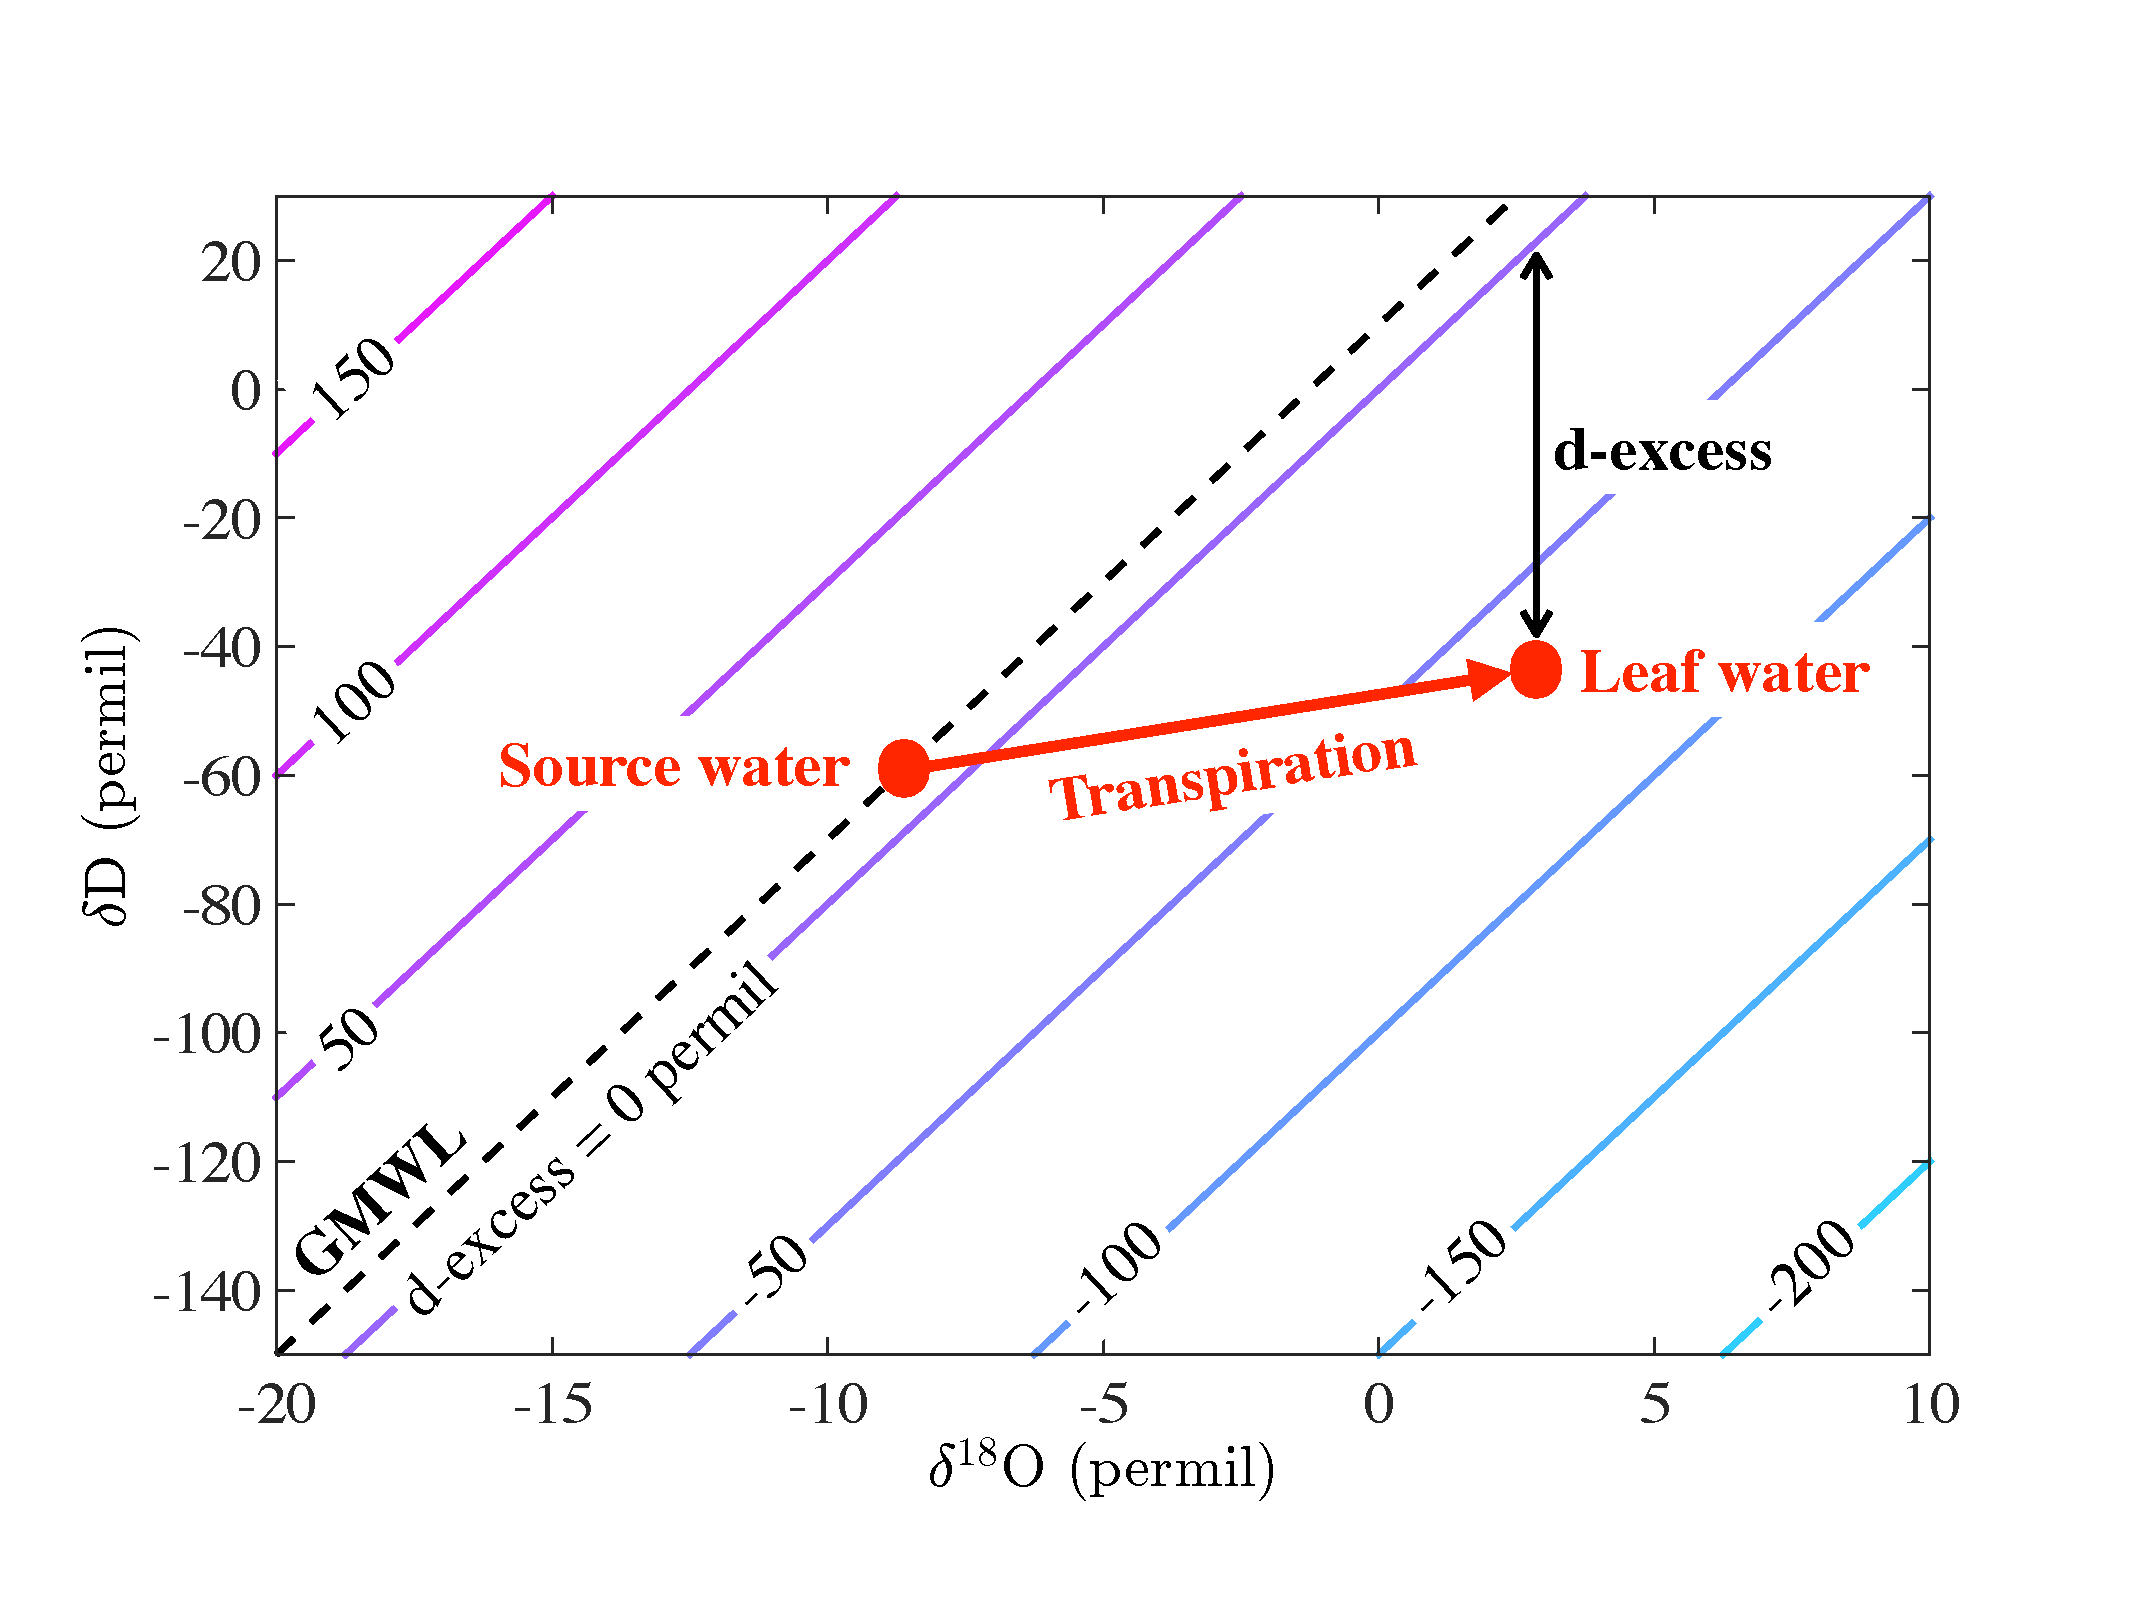
\includegraphics[width=0.7\textwidth]{d18_dD_Concept_Final.pdf}
		\caption{}\label{d18O_dD_Concept}
	\end{figure}
\end{center}
\begin{center}
	\begin{figure}
		\centering
		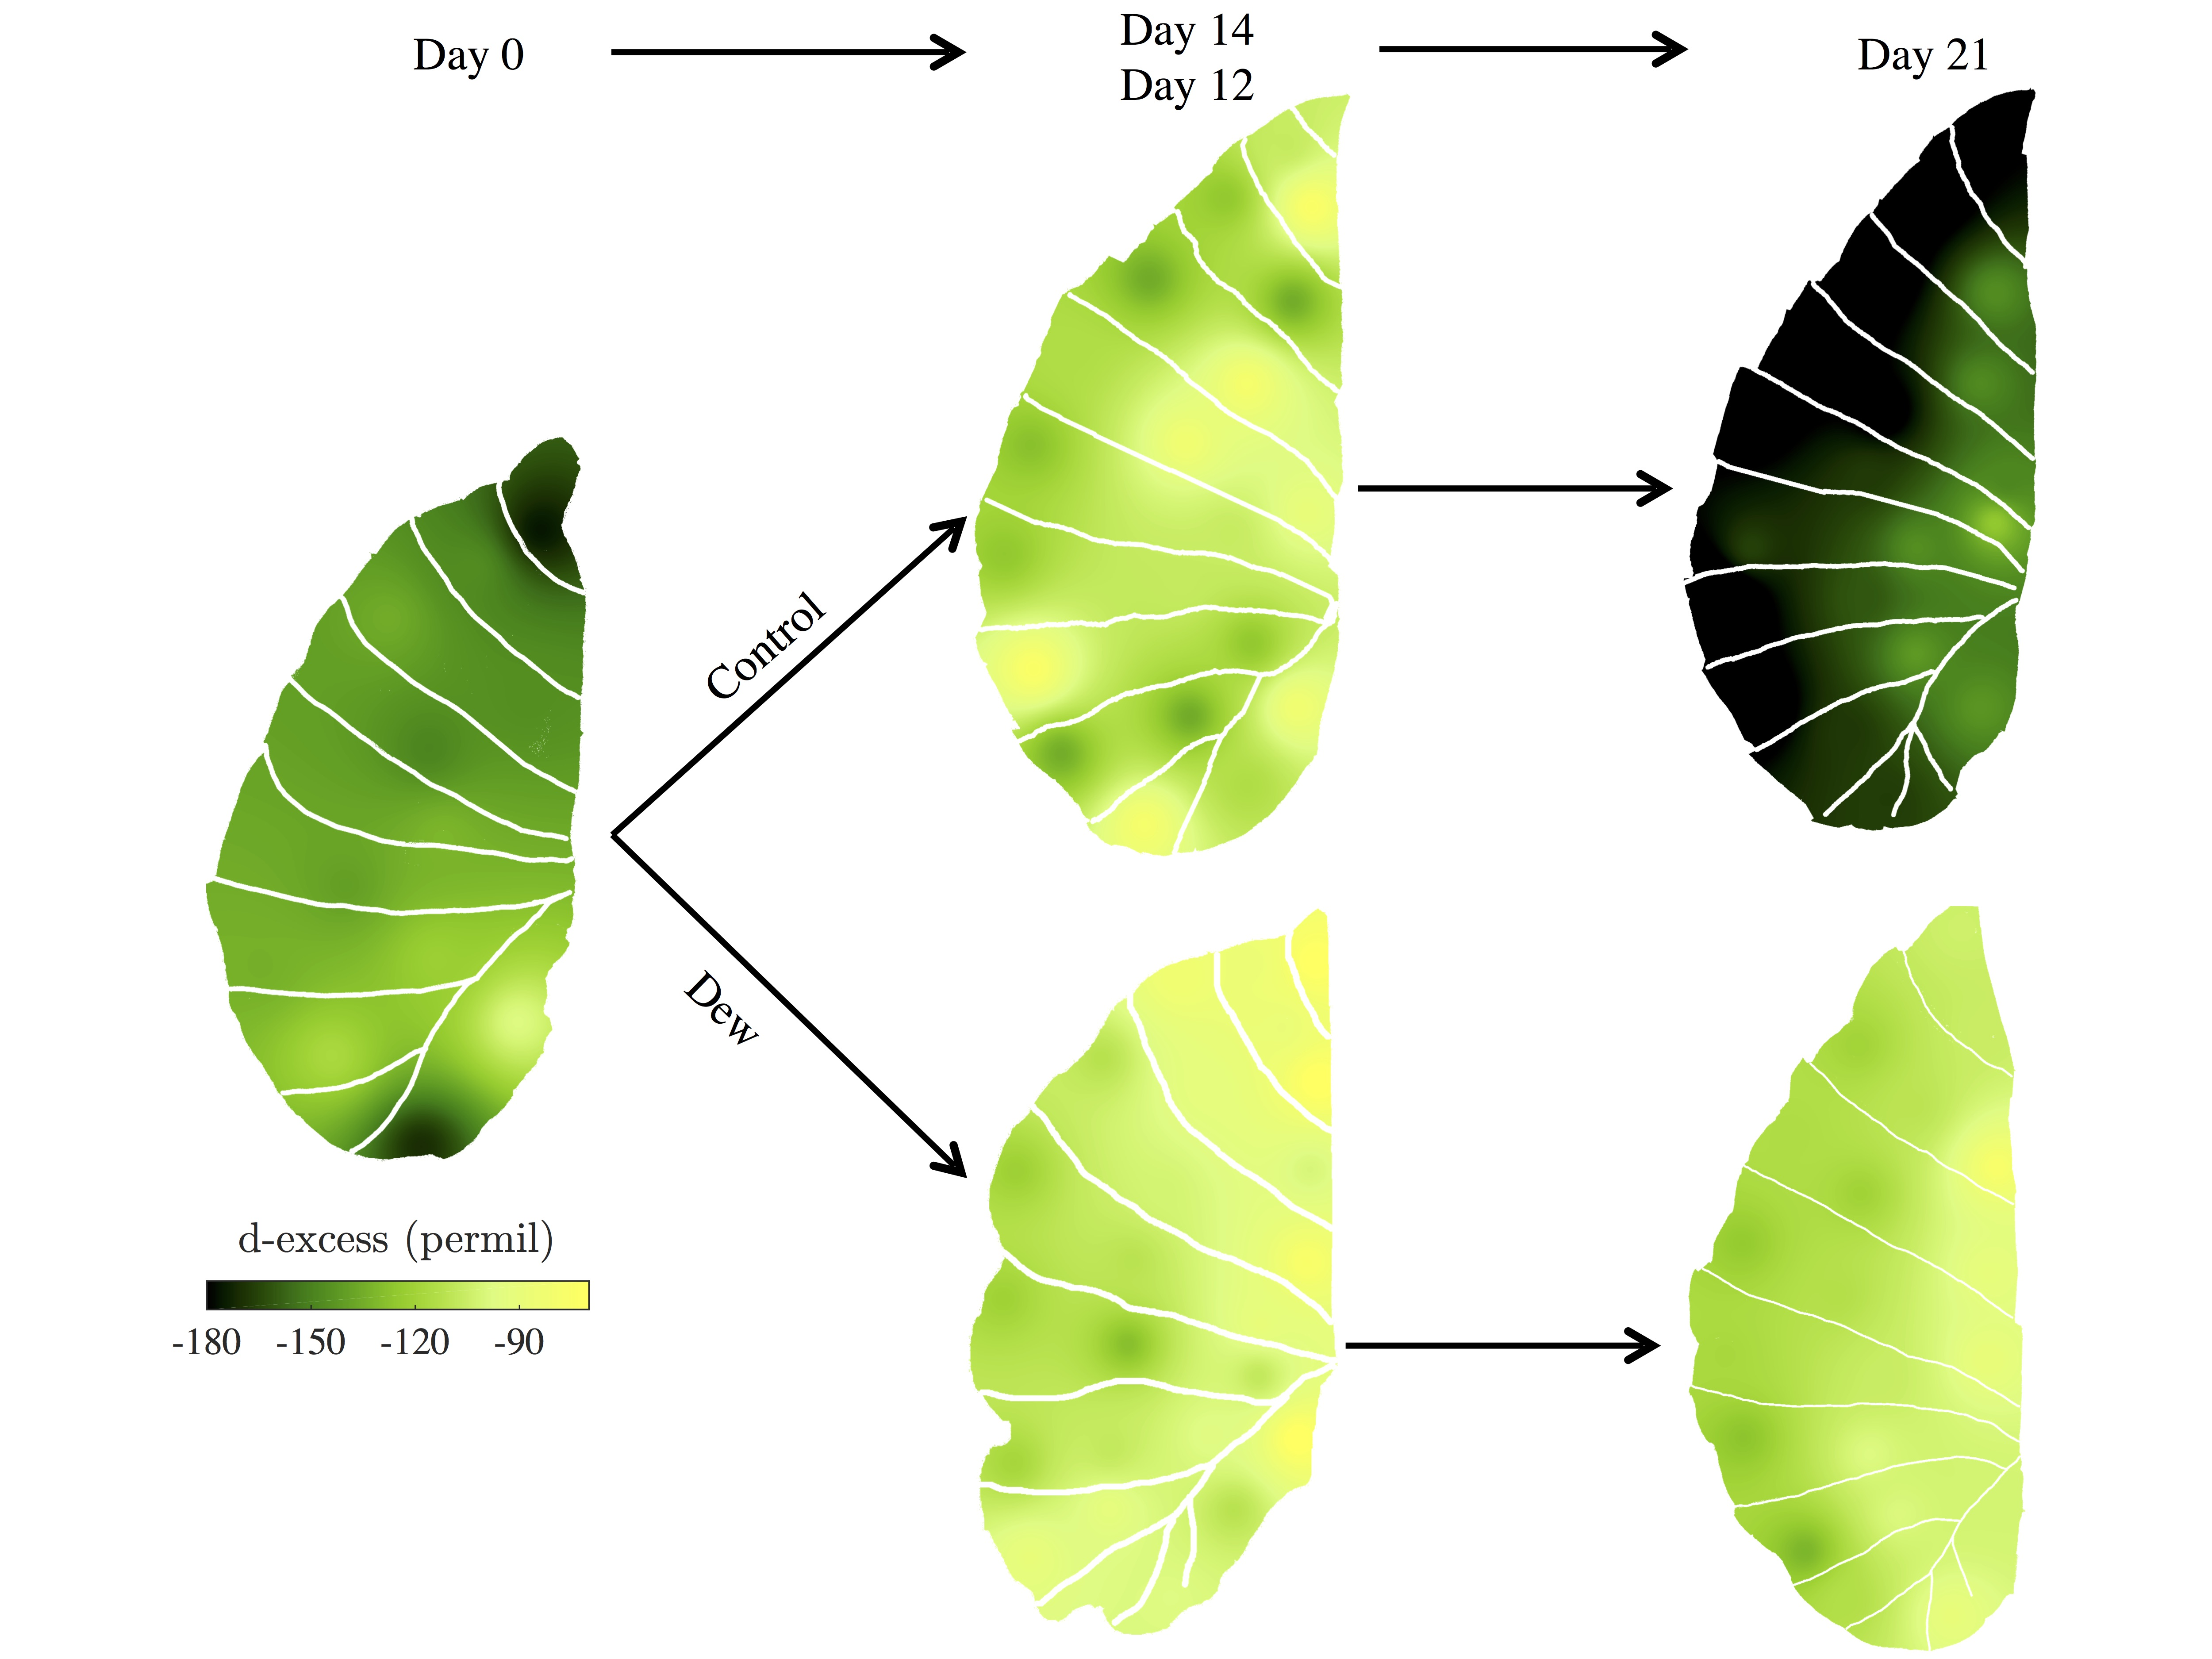
\includegraphics[width=\textwidth]{Final_d_excess_Plot_LowQuality.jpg}
		\caption{}\label{expe1A}
	\end{figure}
\end{center}

\begin{center}
	\begin{figure}
		\centering
		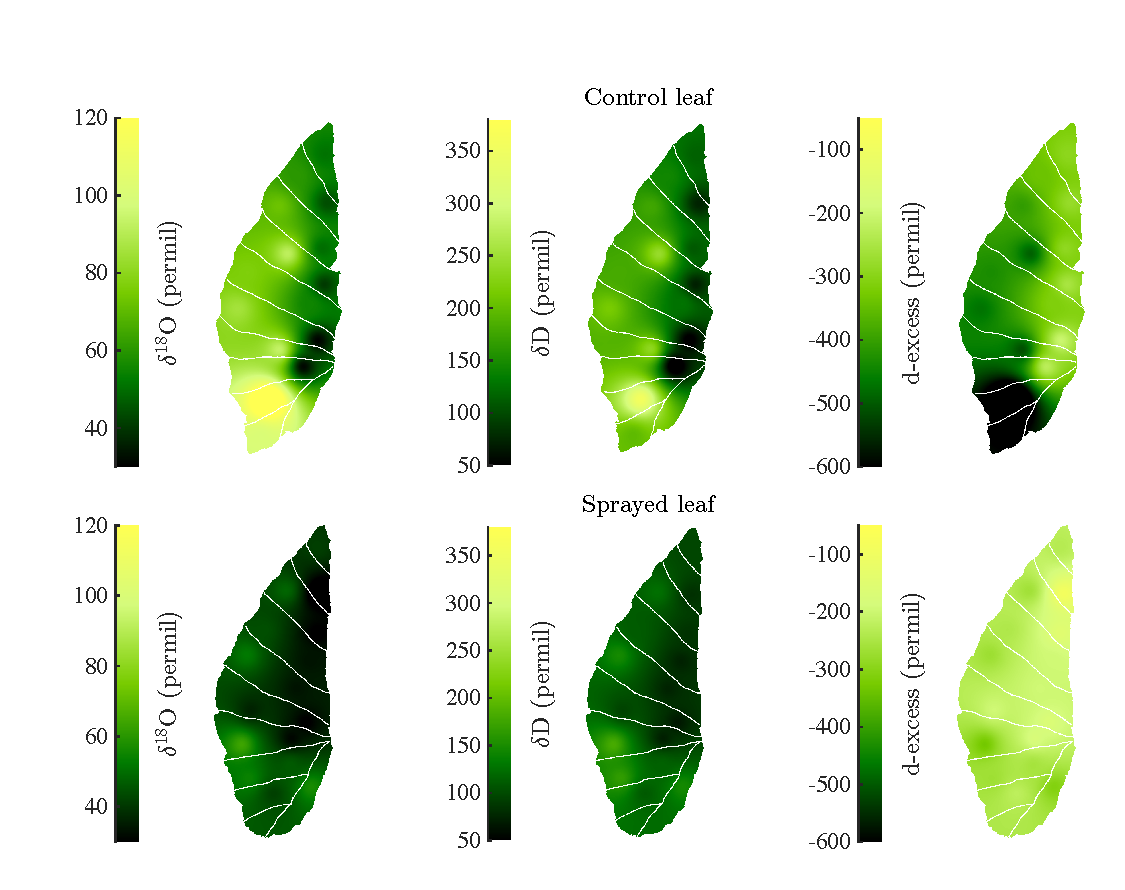
\includegraphics[width=0.9\textwidth]{Dec1stFinal.pdf}
		\caption{}\label{expe1B}
	\end{figure}
\end{center}
\begin{center}
	\begin{figure}
		\centering
		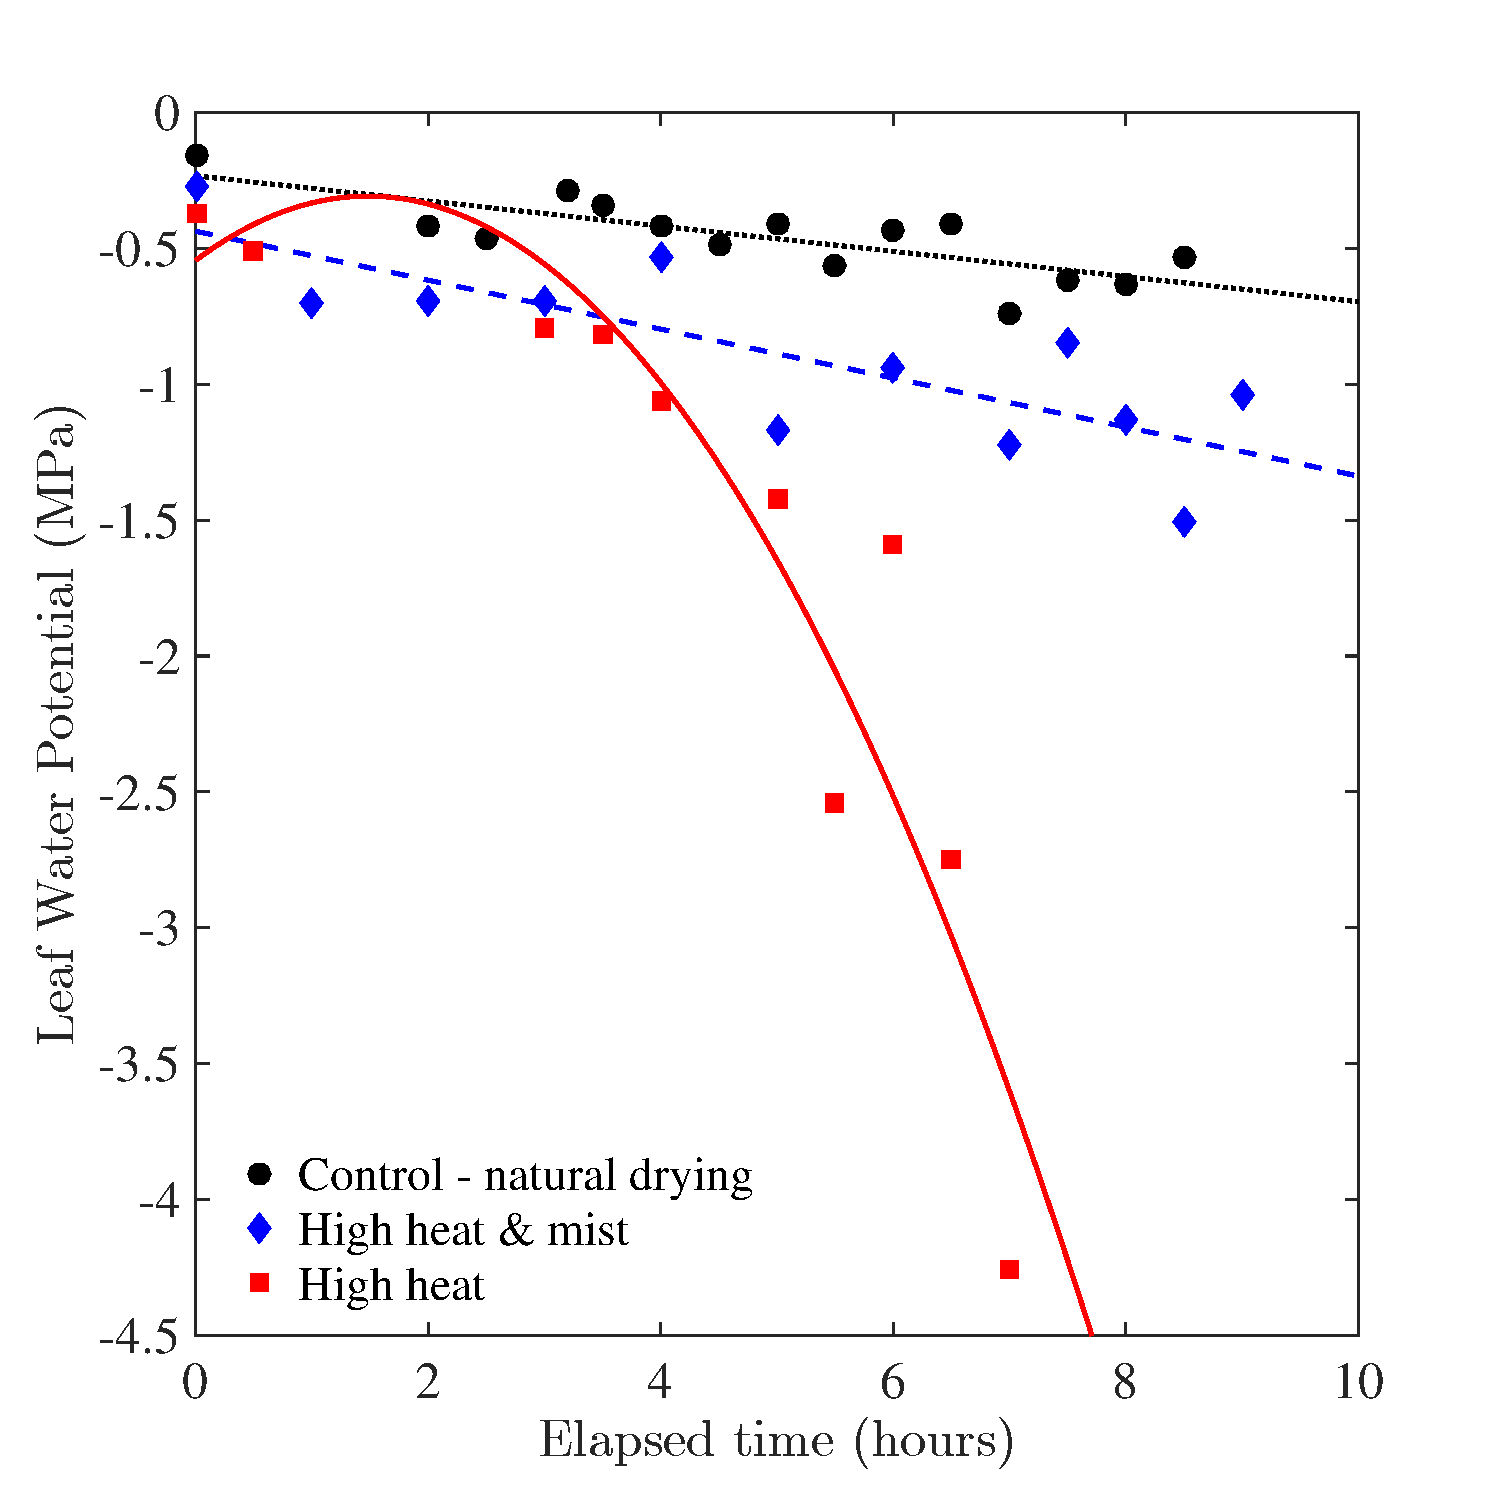
\includegraphics[width=0.5\textwidth]{Dryout_Expe_Compact.pdf}
		\caption{}\label{expe2}
	\end{figure}
\end{center}

\begin{center}
	\begin{figure}
		\centering
		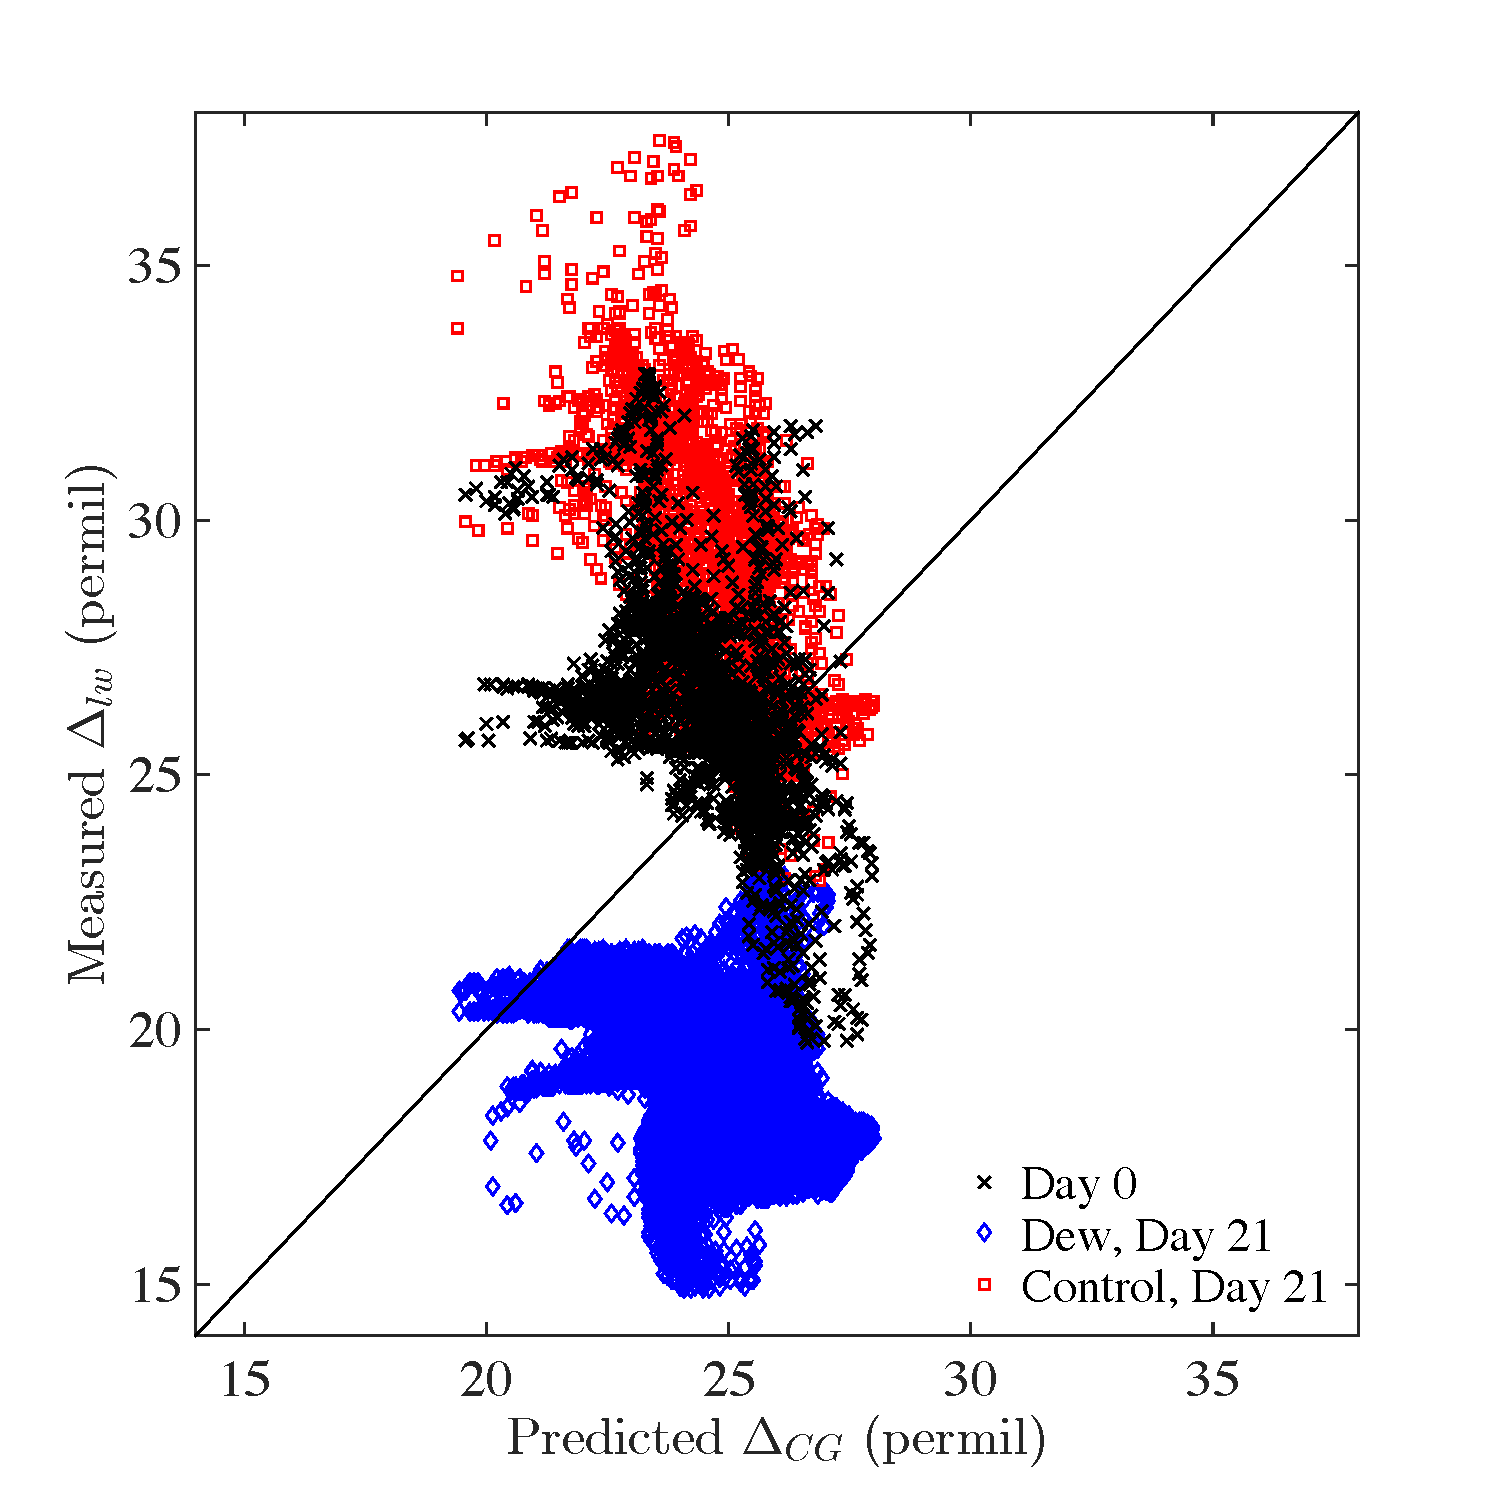
\includegraphics[width=0.5\textwidth]{CGless.pdf}
		\caption{}\label{CG}
	\end{figure}
\end{center}

\begin{center}
	\begin{figure}
		\centering
		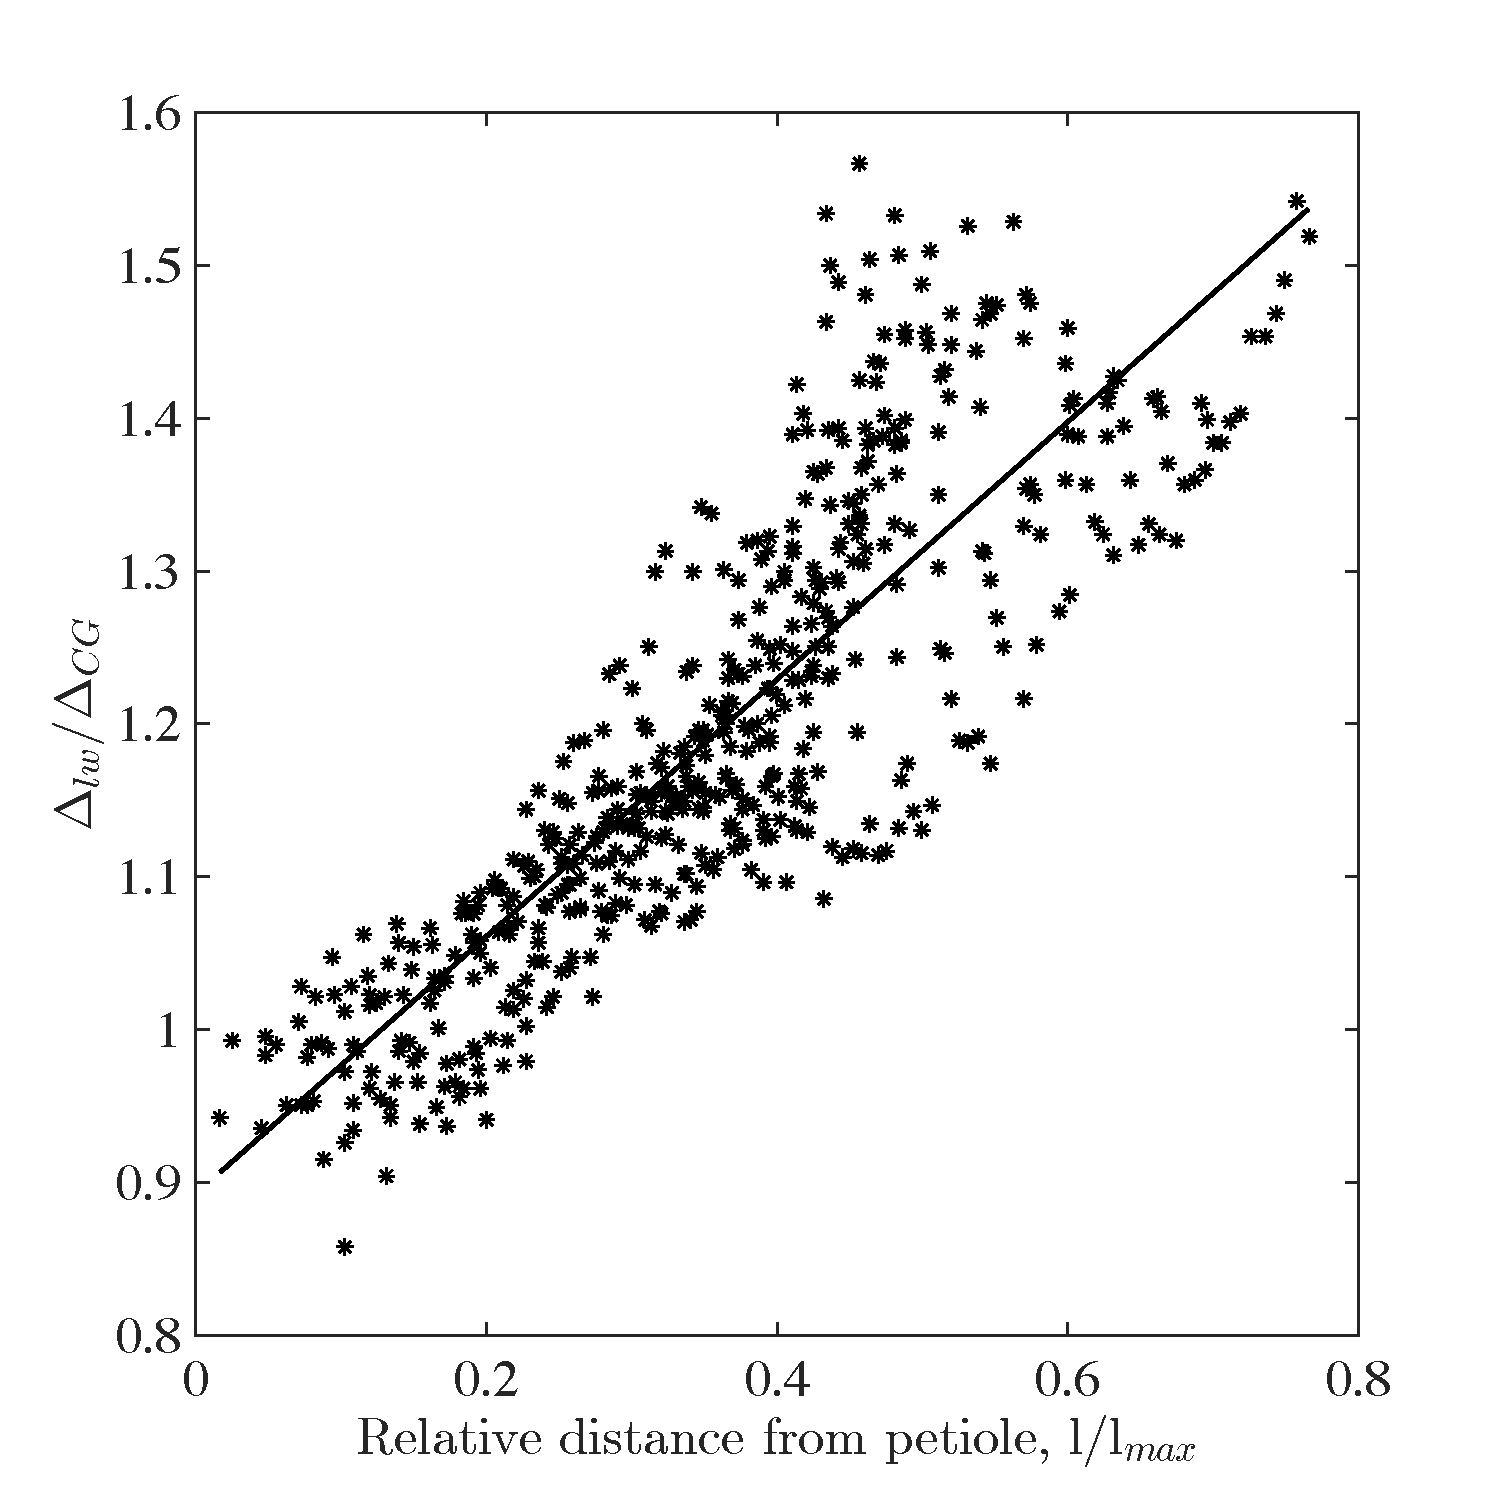
\includegraphics[width=0.5\textwidth]{CG_distance.pdf}
		\caption{}\label{CGdist}
	\end{figure}
\end{center}

\begin{center}
	\begin{figure}
		\centering
		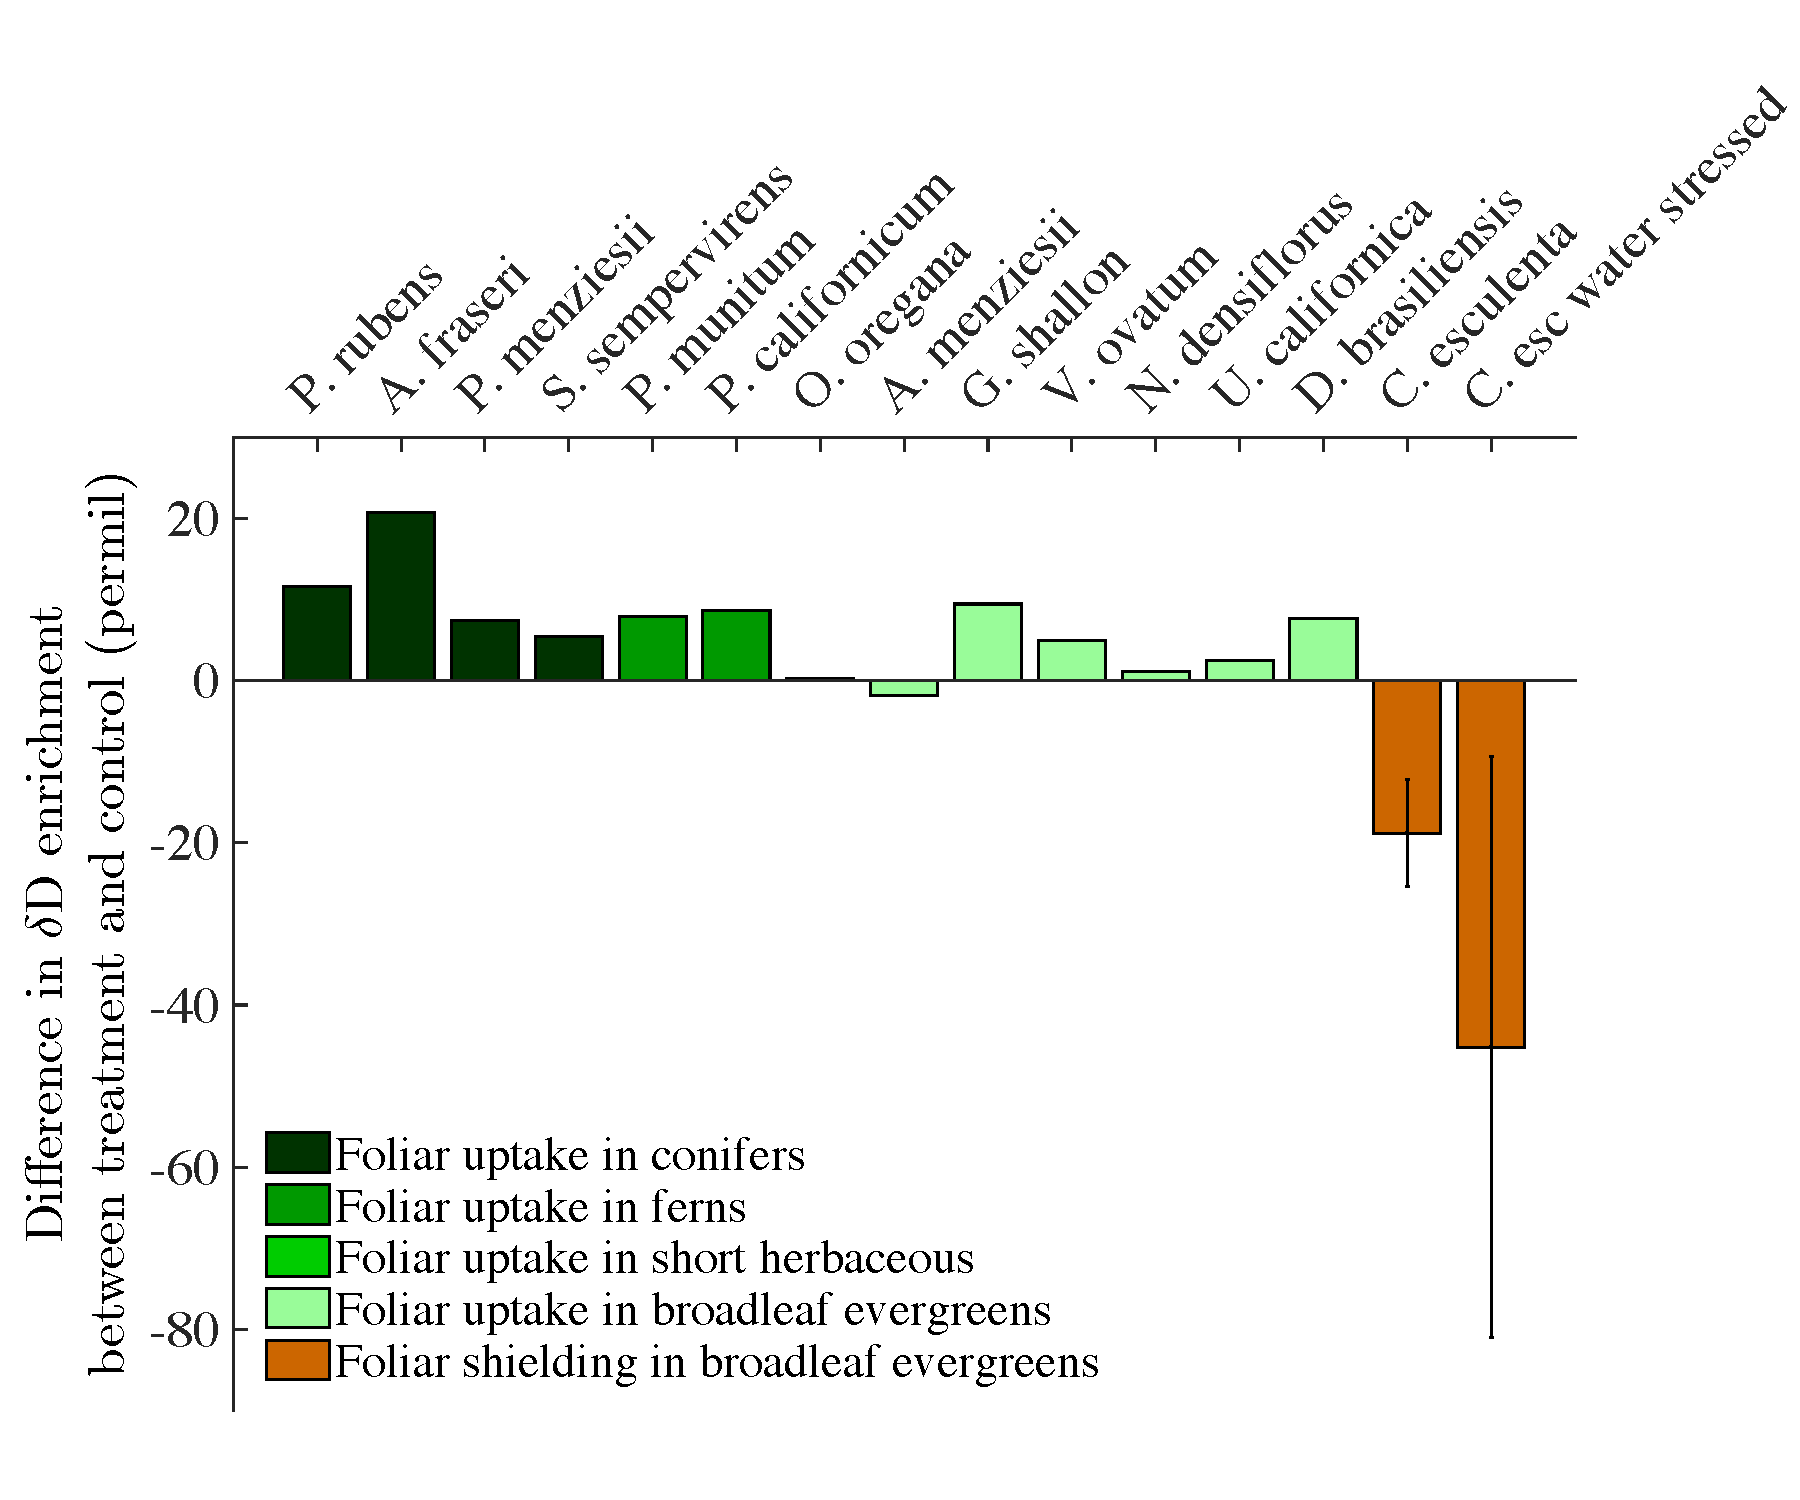
\includegraphics[width=0.7\textwidth]{Bar_Plot_FU_VS_FShielding.pdf}
		\caption{}\label{FU_VS_FS}
	\end{figure}
\end{center}
\clearpage

%----------------------------------------------------------------------------------------
%Supplemental Information
%----------------------------------------------------------------------------------------
\subsection*{Supplemental Information}

\textbf{Article title:} The impacts of dew-induced foliar shielding on the energy, water and isotope balance of leaves\\
~\\
\textbf{Authors:} Cynthia Gerlein-Safdi, Craig James Sinkler, Kelly Krispin Caylor\\
~\\
The following Supporting Information is available for this article:\\
\textbf{Fig. \ref{expe1A2H}}: Interpolated maps showing the $\delta$D of the leaves analyzed in Experiment 1A.\\
\textbf{Fig. \ref{expe1A18O}}: Interpolated maps showing the $\delta^{\text{18}}$O of the leaves analyzed in Experiment 1A.\\

%%%%%%%%%% Merge with supplemental materials %%%%%%%%%%
%%%%%%%%%% Prefix a "S" to all equations, figures, tables and reset the counter %%%%%%%%%%
\setcounter{equation}{0}
\setcounter{figure}{0}
\setcounter{table}{0}
\setcounter{page}{1}
%\makeatletter
\renewcommand{\theequation}{S\arabic{equation}}
\renewcommand{\thefigure}{S\arabic{figure}}

\begin{center}
	\begin{figure}[h!]
		\centering
		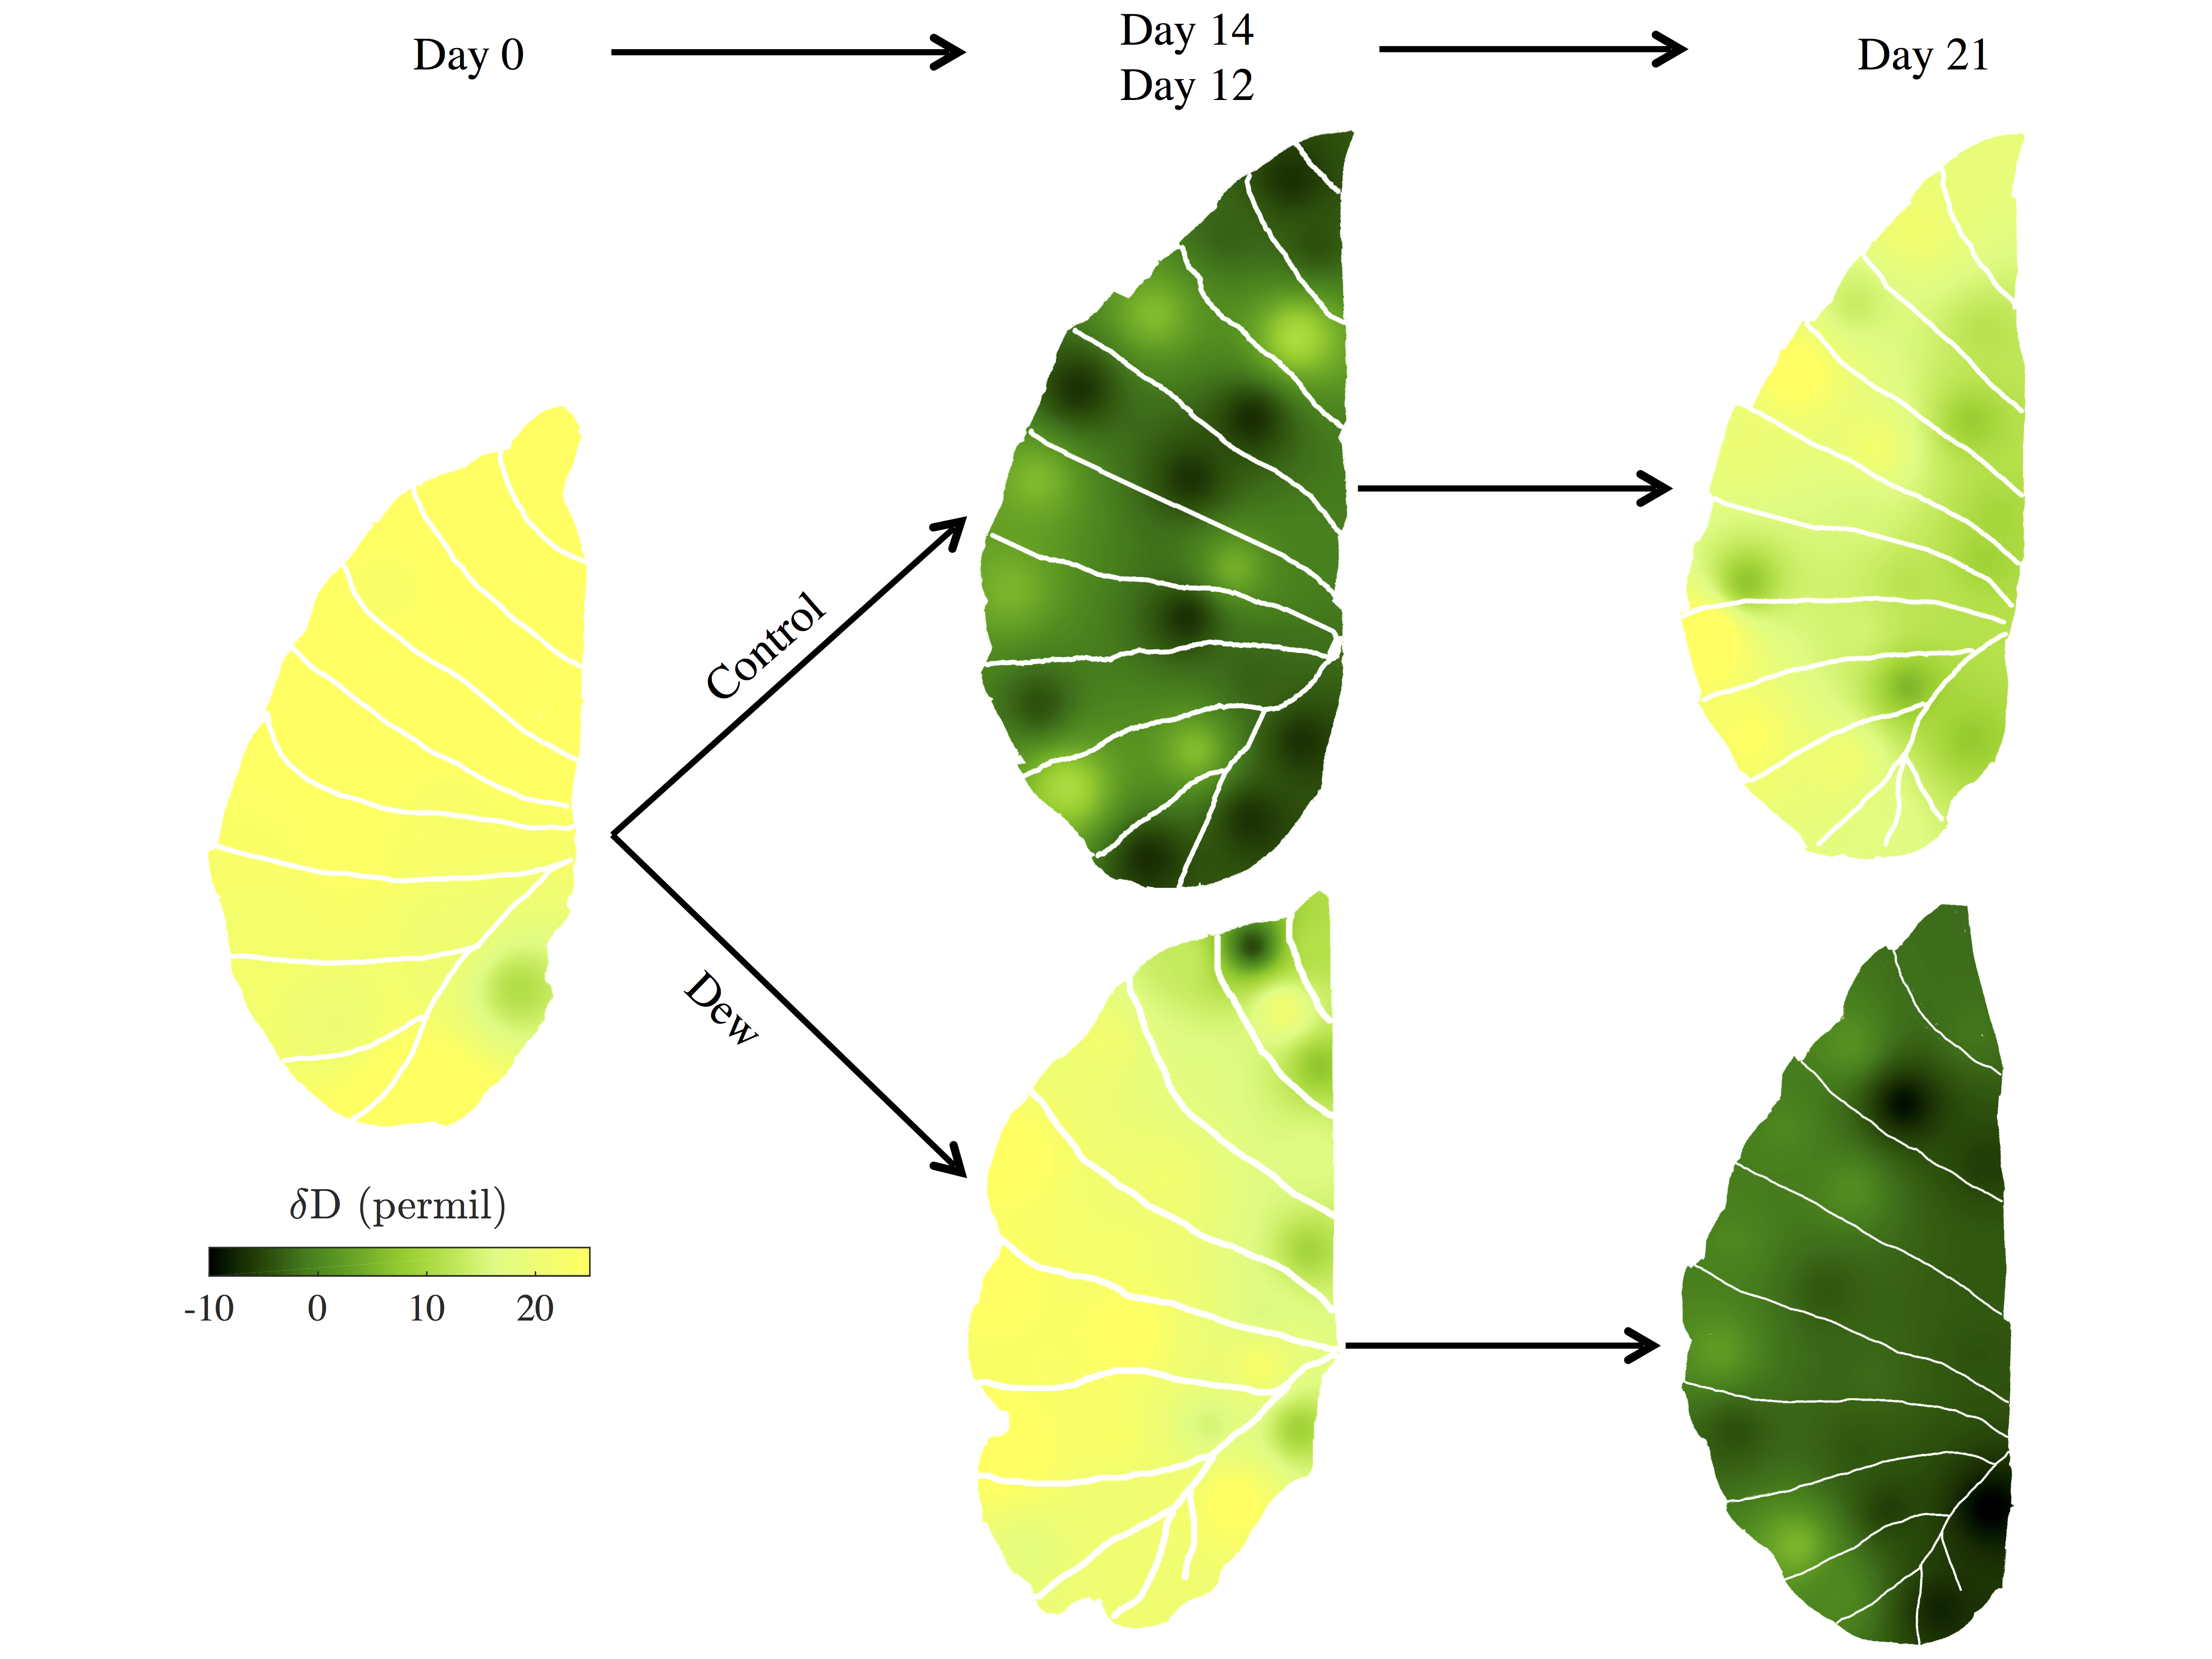
\includegraphics[width=\textwidth]{Final_2H_Plot_GoodQ.jpg}
		\caption{Maps of the spacial distribution of $\delta$D of five \textit{Colocasia esculenta} leaves collected throughout Experiment 1A. The maps were obtained by inverse distance interpolation of 12 to 25 sampling points analyzed on the Picarro Induction Module. All leaves are c. 38~cm long. \textbf{Left:} initial leaf collected on day 0. \textbf{Top row:} leaves collected on day 14 (center) and 21 (far right) from the control. \textbf{Bottom row:} leaves collected on day 12 (center) and 21 (far right) from the sprayed treatment, where the leaves were sprayed with isotopically enriched water ($\delta^{18}$O~$\simeq$~8.85~\textperthousand, $\delta$D~$\simeq$~737.64~\textperthousand) every two days. The color scheme is the same for all rows.}\label{expe1A2H}
	\end{figure}
\end{center}
\begin{center}
	\begin{figure}[h!]
		\centering
		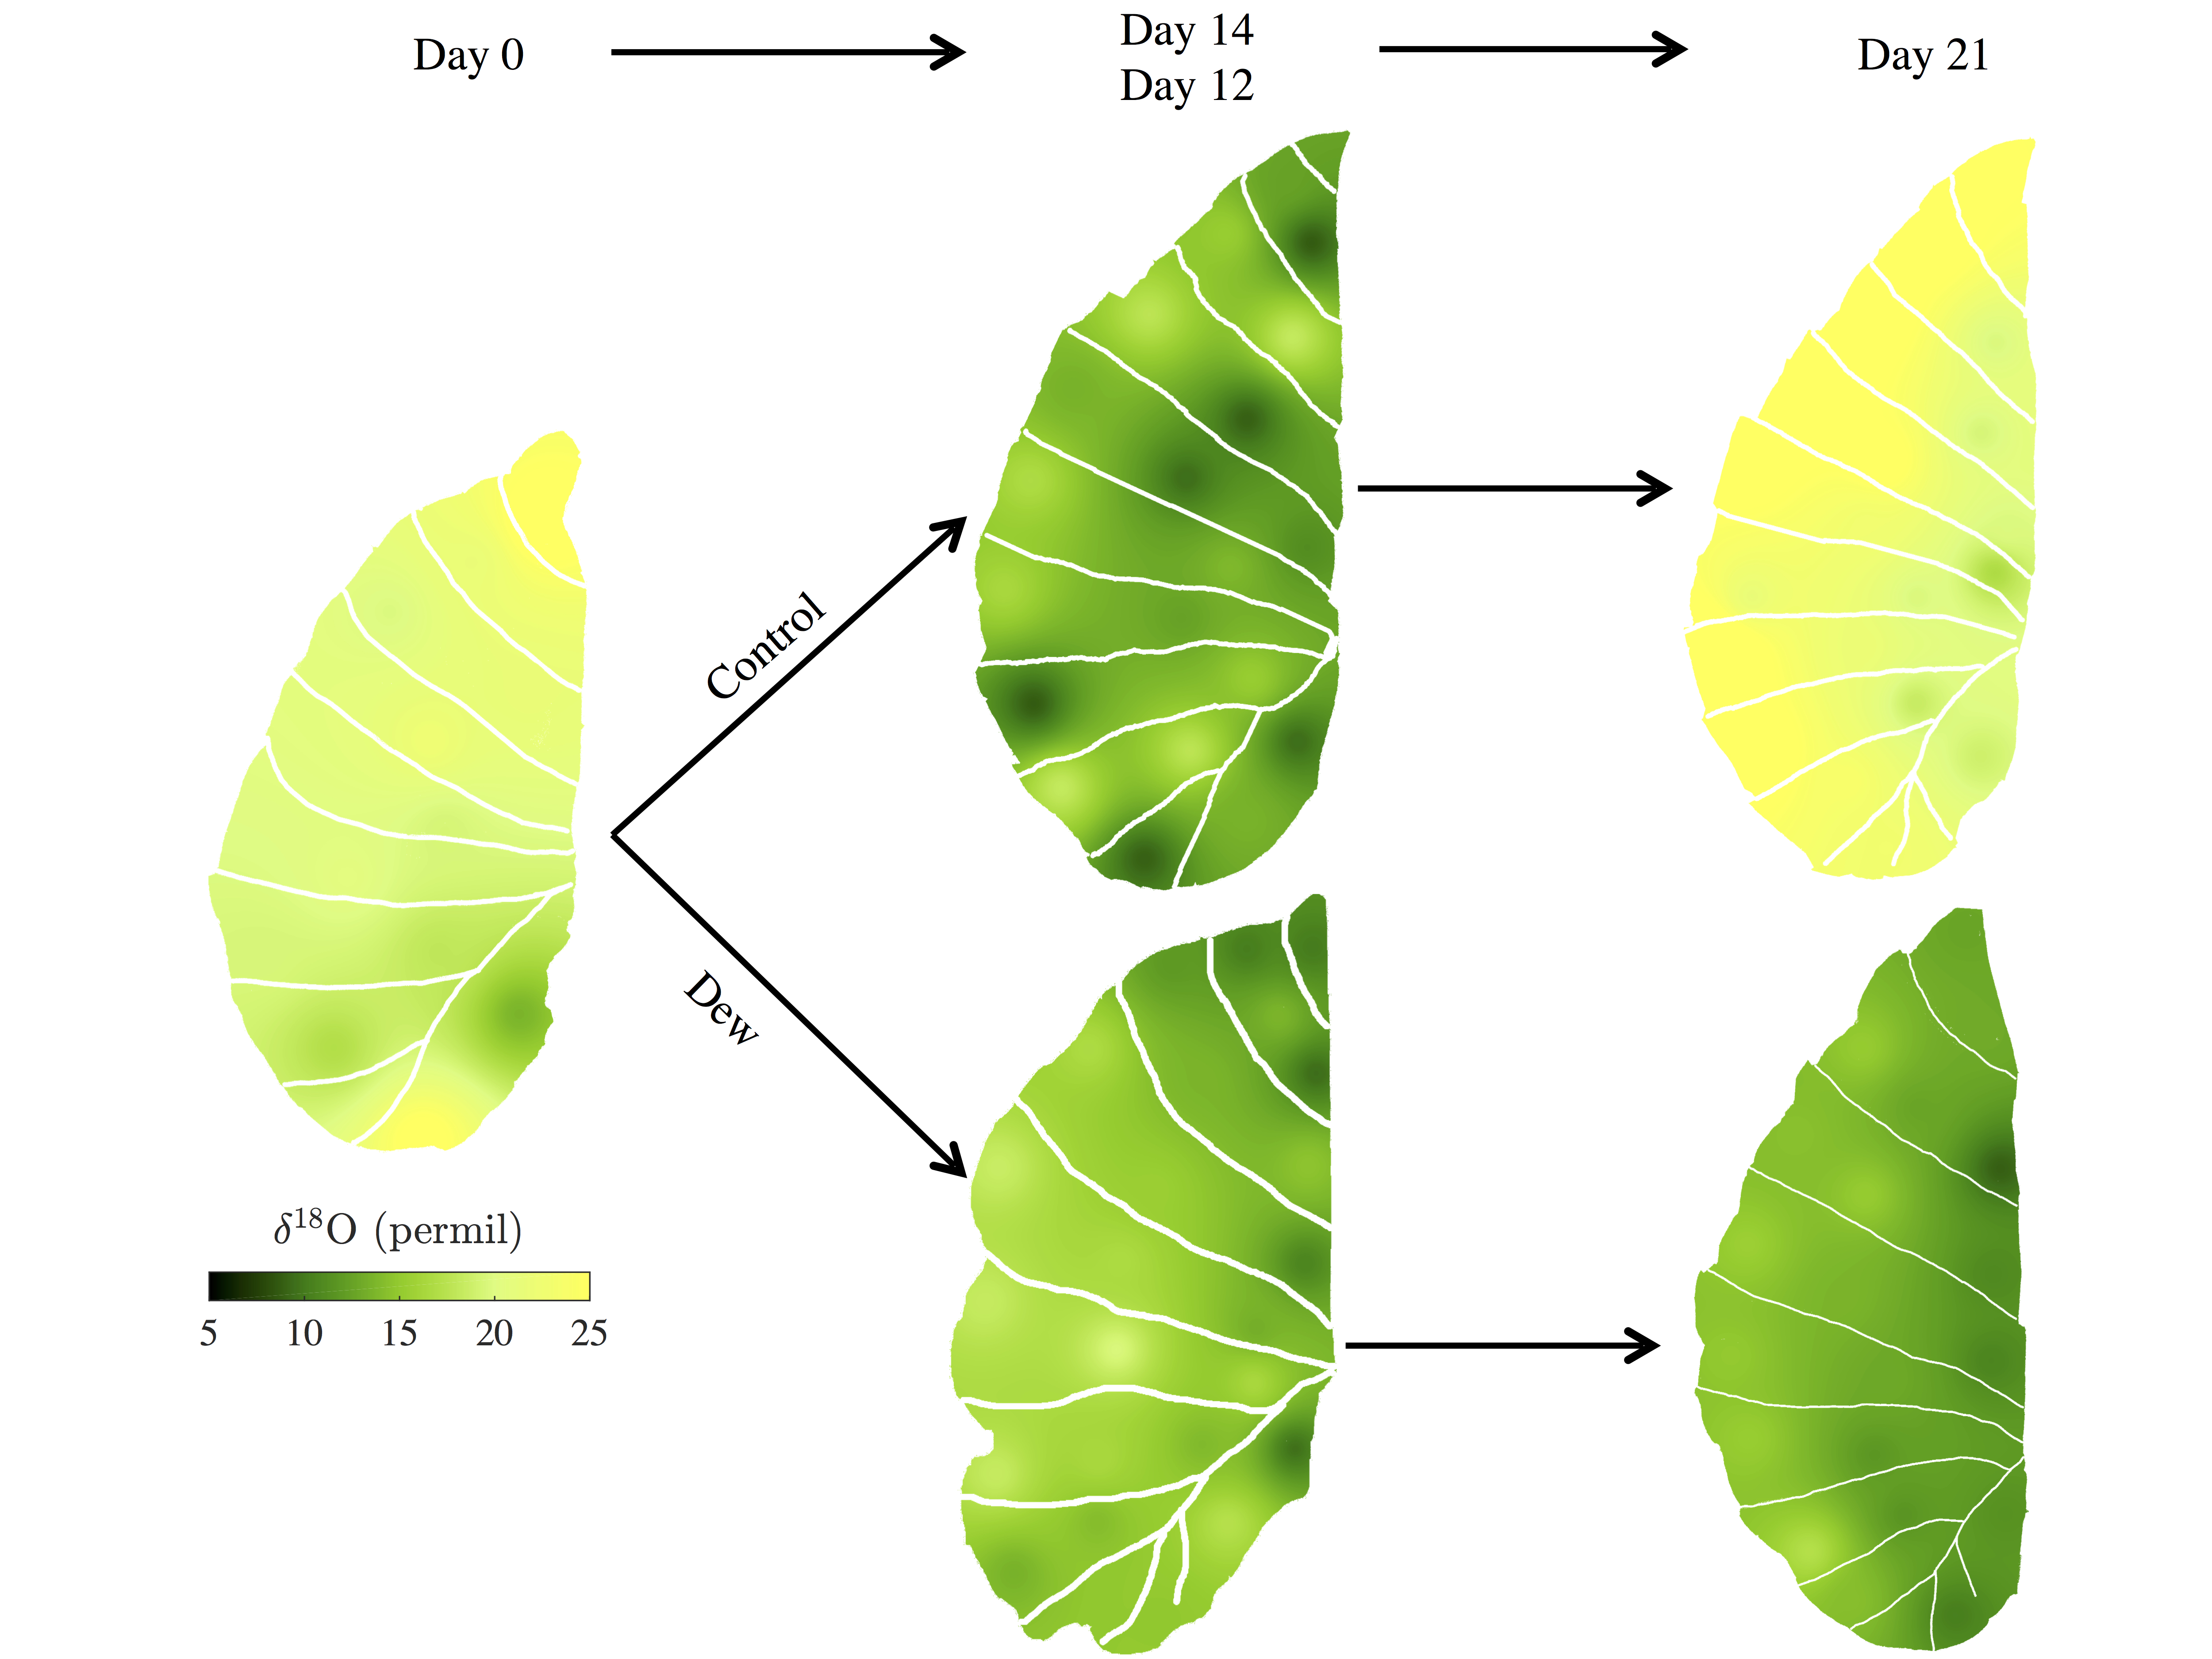
\includegraphics[width=\textwidth]{Final_18O_Plot_GoodQ.jpg}
		\caption{Maps of the spacial distribution of $\delta^{\text{18}}$O of five \textit{Colocasia esculenta} leaves collected throughout Experiment 1A. The maps were obtained by inverse distance interpolation of 12 to 25 sampling points analyzed on the Picarro Induction Module. All leaves are c. 38~cm long. \textbf{Left:} initial leaf collected on day 0. \textbf{Top row:} leaves collected on day 14 (center) and 21 (far right) from the control. \textbf{Bottom row:} leaves collected on day 12 (center) and 21 (far right) from the sprayed treatment, where the leaves were sprayed with isotopically enriched water ($\delta^{18}$O~$\simeq$~8.85~\textperthousand, $\delta$D~$\simeq$~737.64~\textperthousand) every two days. The color scheme is the same for all rows.}\label{expe1A18O}
	\end{figure}
\end{center}
%\begin{center}
%	\begin{figure}
%		\centering
%		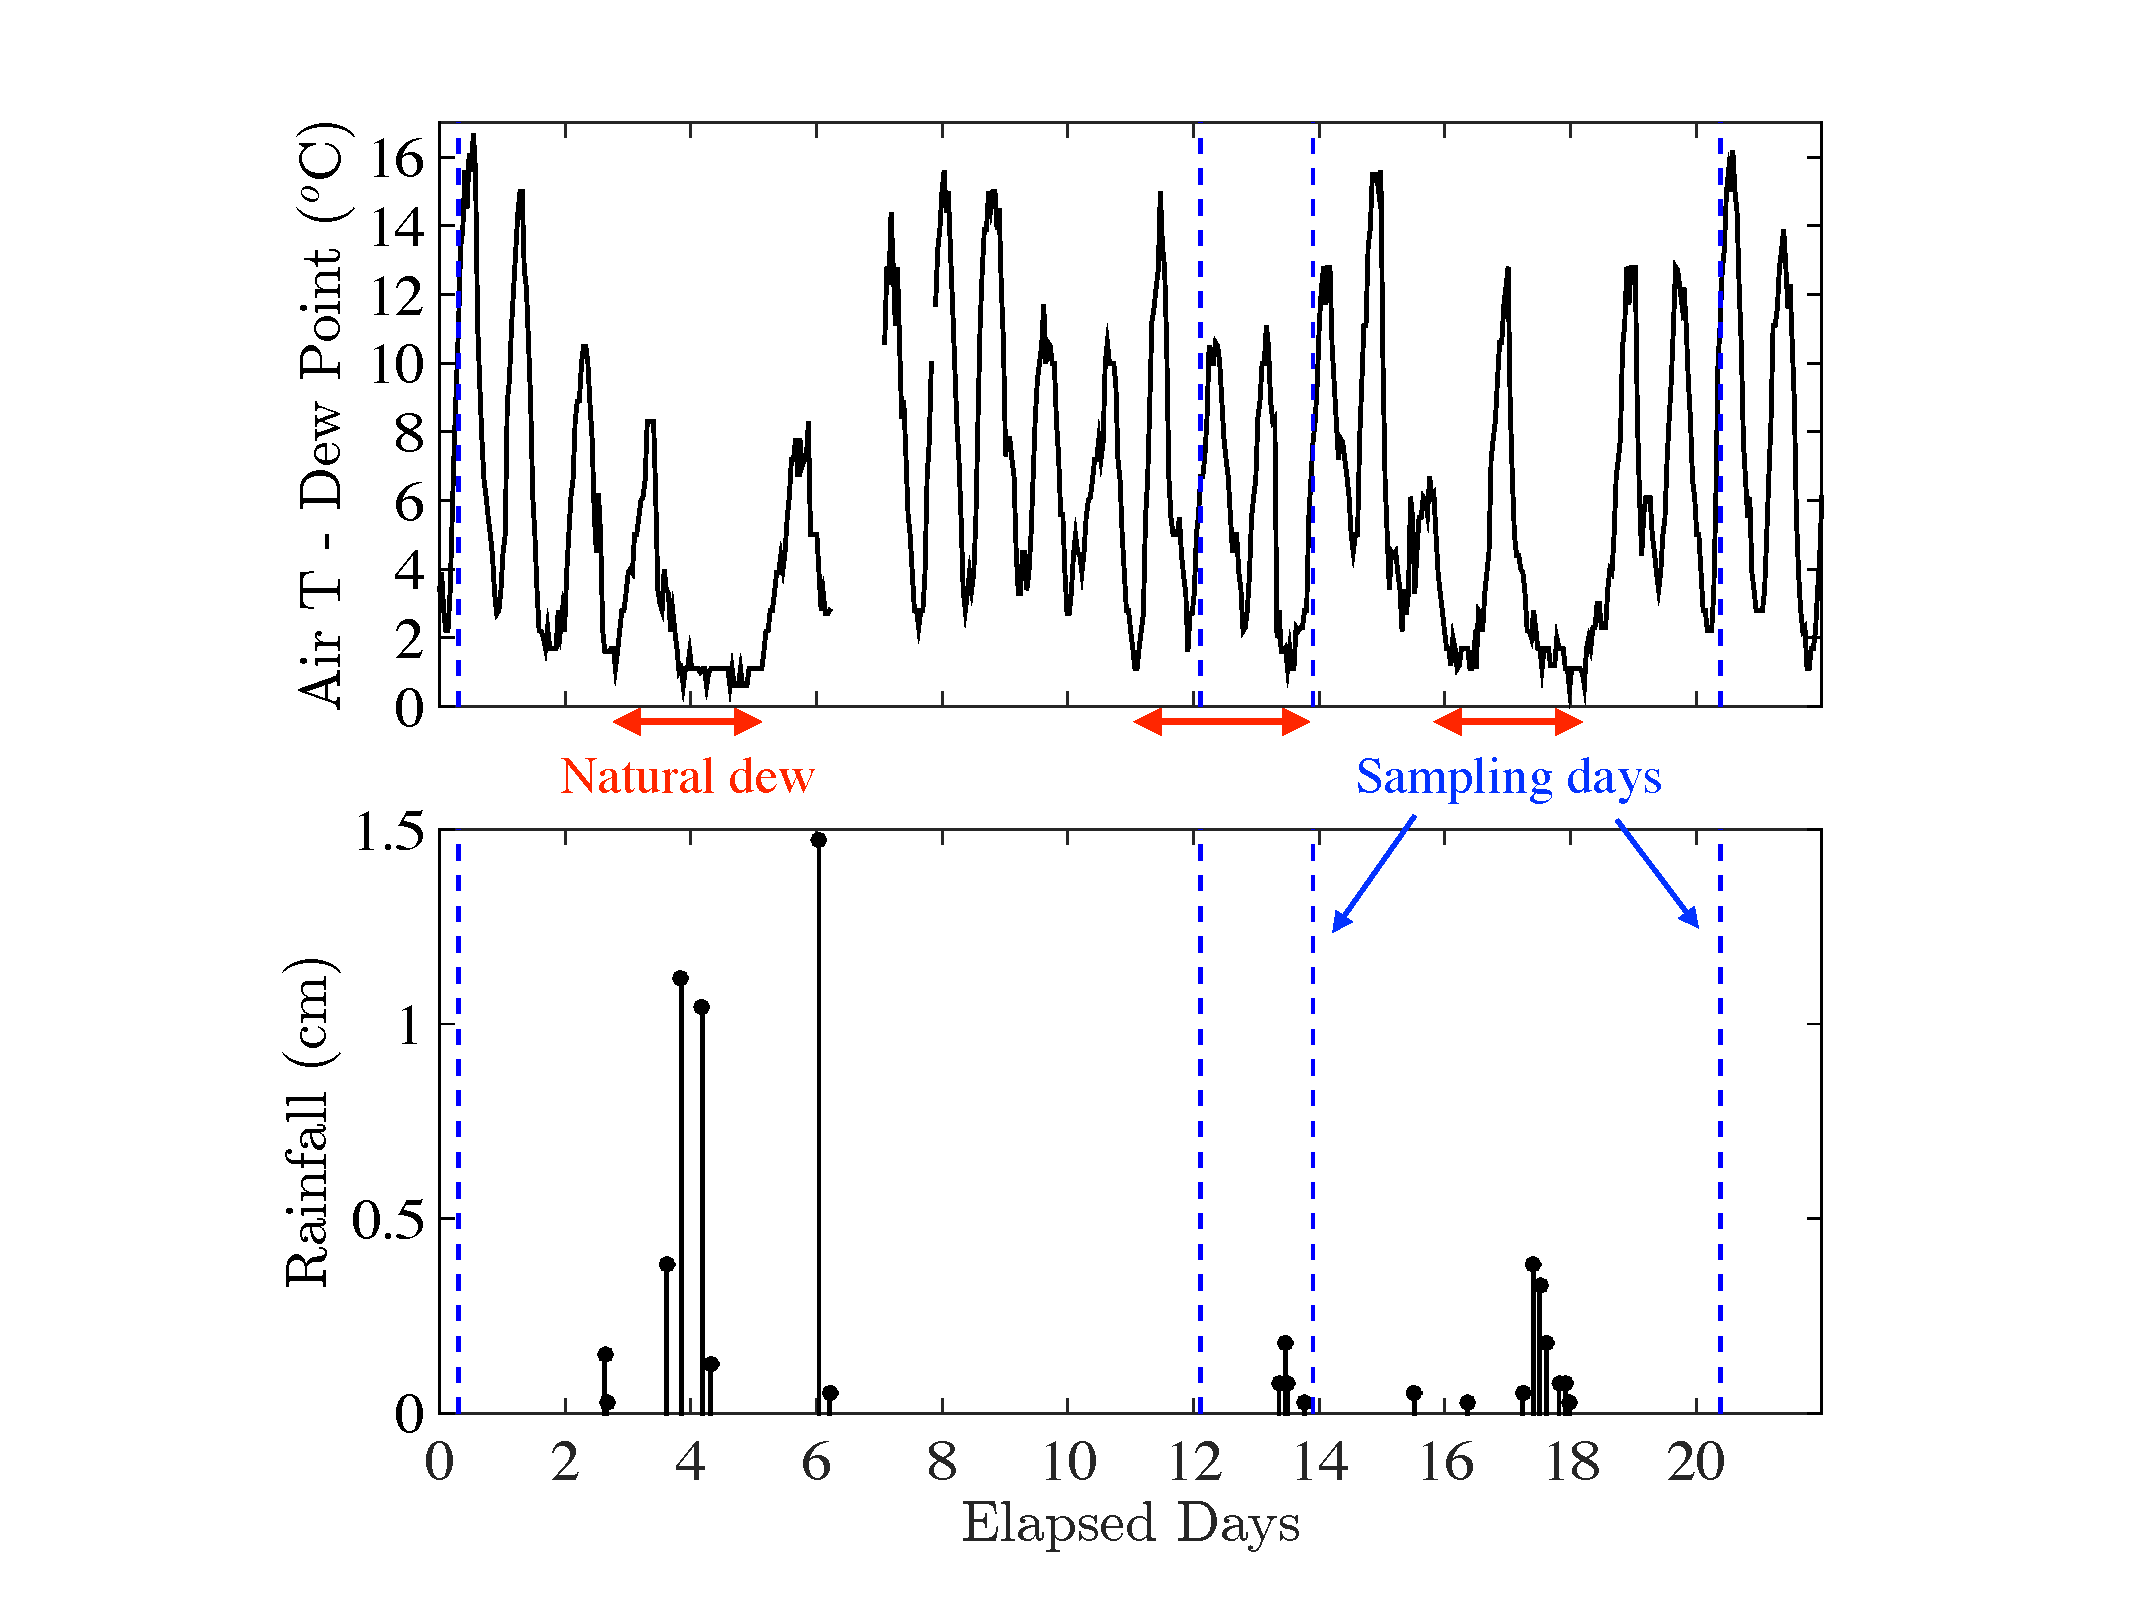
\includegraphics[width=0.8\textwidth]{Experiment_DewPoint_T_Annotated.pdf}
%		\caption{\textbf{Top panel:} Difference between the air and the dew point temperature over the course of the experiment ($^{\text{o}}$C). \textbf{Bottom panel:} Rainfall (cm) over the course of the experiment. The blue dashed vertical lines mark the days of collection: the initial leaf was collected on day 0, leaves from the dew treatment were collected on days 12 and 21 and leaves from the control were collected on days 14 and 21. Red horizontal arrows indicate days when the leaves most likely experienced natural dew deposition because of the local air temperature and relative humidity under the sheltered area. The collection of the first control leaf happened after a series of small rain events and four nights of natural dew formation.}\label{dewpoint}
%	\end{figure}
%\end{center}
\end{document}
